\documentclass[11pt]{article}
\usepackage[margin=1.15in]{geometry}
\usepackage{xcolor}
\usepackage{amsmath,amssymb,amsthm,mathtools,booktabs,longtable,graphicx,enumitem,hyperref,cleveref,microtype,xurl,array}
\graphicspath{{../figures/}}
\hypersetup{colorlinks=true,linkcolor=blue!50!black,citecolor=blue!50!black,urlcolor=blue!50!black,
 pdftitle={The Geometry of Generation in the UNNS Substrate: A Mathematical Synthesis},
 pdfauthor={UNNS Research Collective},
 pdfsubject={Manuscript IV of the GEO-HD-1 programme: synthesis of generation, ancestry and evolving occurrence geometry},
 pdfkeywords={arithmetic generation; endpoint projection; occurrence set; divisor-interval complex; swap classes; collective map; obstruction; factorization}}
\usepackage{aliascnt}
\theoremstyle{plain}
\newtheorem{theorem}{Theorem}[section]
\newaliascnt{lemma}{theorem}\newtheorem{lemma}[lemma]{Lemma}\aliascntresetthe{lemma}
\newaliascnt{proposition}{theorem}\newtheorem{proposition}[proposition]{Proposition}\aliascntresetthe{proposition}
\newaliascnt{corollary}{theorem}\newtheorem{corollary}[corollary]{Corollary}\aliascntresetthe{corollary}
\theoremstyle{definition}
\newaliascnt{definition}{theorem}\newtheorem{definition}[definition]{Definition}\aliascntresetthe{definition}
\newaliascnt{example}{theorem}\newtheorem{example}[example]{Example}\aliascntresetthe{example}
\newaliascnt{problem}{theorem}\newtheorem{problem}[problem]{Problem}\aliascntresetthe{problem}
\theoremstyle{remark}
\newaliascnt{remark}{theorem}\newtheorem{remark}[remark]{Remark}\aliascntresetthe{remark}
\crefname{theorem}{Theorem}{Theorems}\crefname{lemma}{Lemma}{Lemmas}\crefname{proposition}{Proposition}{Propositions}
\crefname{corollary}{Corollary}{Corollaries}\crefname{definition}{Definition}{Definitions}\crefname{example}{Example}{Examples}
\crefname{section}{Section}{Sections}\crefname{figure}{Figure}{Figures}\Crefname{figure}{Figure}{Figures}
\crefname{appendix}{Appendix}{Appendices}\crefname{problem}{Problem}{Problems}\crefname{remark}{Remark}{Remarks}\crefname{table}{Table}{Tables}
% ---- notation
\newcommand{\Z}{\mathbb Z}\newcommand{\Q}{\mathbb Q}\newcommand{\N}{\mathbb N}
\newcommand{\lcm}{\operatorname{lcm}}
\newcommand{\Gr}{\mathrm{Gr}}
\newcommand{\Kmove}{K_{\mathrm{move}}}
\newcommand{\Hist}{\mathrm{Hist}}
\newcommand{\Endp}{\operatorname{end}}
\newcommand{\Dset}{D}
\newcommand{\SIV}[1]{\textsc{SIV-P#1}}
% ---- source references resolved from the v0.4 manuscripts (generated file)
% generated by scripts/gen_xref.py from the v0.4 .aux and .prov files of Papers I-III
\makeatletter
\expandafter\def\csname xr@I-prop:fibre\endcsname{Proposition~2.1}
\expandafter\def\csname xr@I-def:cell\endcsname{Definition~2.3}
\expandafter\def\csname xr@I-lem:intrinsic\endcsname{Lemma~2.4}
\expandafter\def\csname xr@I-prop:E22\endcsname{Proposition~3.1}
\expandafter\def\csname xr@I-thm:P2T1\endcsname{Theorem~3.2}
\expandafter\def\csname xr@I-cor:denominators\endcsname{Corollary~3.3}
\expandafter\def\csname xr@I-lem:orderrule\endcsname{Lemma~3.4}
\expandafter\def\csname xr@I-prop:fibre-vs-lattice\endcsname{Proposition~3.5}
\expandafter\def\csname xr@I-prop:corpus\endcsname{Proposition~3.6}
\expandafter\def\csname xr@I-lem:regionG\endcsname{Lemma~4.1}
\expandafter\def\csname xr@I-thm:P2T2\endcsname{Theorem~4.2}
\expandafter\def\csname xr@I-thm:cell-transport\endcsname{Theorem~4.3}
\expandafter\def\csname xr@I-prop:E25\endcsname{Proposition~4.4}
\expandafter\def\csname xr@I-thm:E21\endcsname{Theorem~4.5}
\expandafter\def\csname xr@I-cor:threestage\endcsname{Corollary~4.6}
\expandafter\def\csname xr@I-prop:specimen\endcsname{Proposition~4.7}
\expandafter\def\csname xr@I-thm:P2TF1\endcsname{Theorem~4.8}
\expandafter\def\csname xr@I-lem:gap\endcsname{Lemma~5.1}
\expandafter\def\csname xr@I-thm:corner\endcsname{Theorem~5.2}
\expandafter\def\csname xr@I-thm:evensum\endcsname{Theorem~5.4}
\expandafter\def\csname xr@I-cor:E27\endcsname{Corollary~5.5}
\expandafter\def\csname xr@I-thm:E28\endcsname{Theorem~6.1}
\expandafter\def\csname xr@I-prop:E29\endcsname{Proposition~6.2}
\expandafter\def\csname xr@I-prop:topology\endcsname{Proposition~6.3}
\expandafter\def\csname xr@I-thm:laws\endcsname{Theorem~6.4}
\expandafter\def\csname xr@I-lem:L1\endcsname{Lemma~7.1}
\expandafter\def\csname xr@I-lem:T0\endcsname{Lemma~7.2}
\expandafter\def\csname xr@I-prop:Z\endcsname{Proposition~7.3}
\expandafter\def\csname xr@I-lem:LG\endcsname{Lemma~7.4}
\expandafter\def\csname xr@I-thm:planar\endcsname{Theorem~7.5}
\expandafter\def\csname xr@I-cor:CP\endcsname{Corollary~7.7}
\expandafter\def\csname xr@I-prop:scope\endcsname{Proposition~7.8}
\expandafter\def\csname xr@I-thm:D1\endcsname{Theorem~8.1}
\expandafter\def\csname xr@I-thm:C1\endcsname{Theorem~8.2}
\expandafter\def\csname xr@I-cor:C2\endcsname{Corollary~8.3}
\expandafter\def\csname xr@I-prop:C3\endcsname{Proposition~8.5}
\expandafter\def\csname xr@I-thm:F1\endcsname{Theorem~8.6}
\expandafter\def\csname xr@I-prop:census\endcsname{Proposition~8.7}
\expandafter\def\csname xr@I-thm:slab-i\endcsname{Theorem~9.1}
\expandafter\def\csname xr@I-cor:slab-lemma\endcsname{Corollary~9.2}
\expandafter\def\csname xr@I-thm:slab-ii\endcsname{Theorem~9.3}
\expandafter\def\csname xr@I-cor:S3\endcsname{Corollary~9.5}
\expandafter\def\csname xr@I-prop:H1\endcsname{Proposition~10.1}
\expandafter\def\csname xr@I-prop:P4A\endcsname{Proposition~10.2}
\expandafter\def\csname xr@I-thm:hull\endcsname{Theorem~10.3}
\expandafter\def\csname xr@I-thm:P4T2\endcsname{Theorem~10.4}
\expandafter\def\csname xr@I-cor:P4C1\endcsname{Corollary~10.5}
\expandafter\def\csname xr@I-prop:holes\endcsname{Proposition~10.6}
\expandafter\def\csname xr@I-lem:lift\endcsname{Lemma~B.1}
\expandafter\def\csname xr@II-def:select\endcsname{Definition~2.1}
\expandafter\def\csname xr@II-lem:adm\endcsname{Lemma~2.2}
\expandafter\def\csname xr@II-lem:R\endcsname{Lemma~2.3}
\expandafter\def\csname xr@II-def:history\endcsname{Definition~2.4}
\expandafter\def\csname xr@II-thm:predecessors\endcsname{Theorem~3.1}
\expandafter\def\csname xr@II-prop:growth\endcsname{Proposition~3.4}
\expandafter\def\csname xr@II-def:K\endcsname{Definition~4.1}
\expandafter\def\csname xr@II-thm:threshold\endcsname{Theorem~4.2}
\expandafter\def\csname xr@II-cor:P\endcsname{Corollary~4.3}
\expandafter\def\csname xr@II-cor:G\endcsname{Corollary~4.4}
\expandafter\def\csname xr@II-prop:diamond\endcsname{Proposition~4.5}
\expandafter\def\csname xr@II-prop:sat\endcsname{Proposition~4.6}
\expandafter\def\csname xr@II-def:swapgraph\endcsname{Definition~5.1}
\expandafter\def\csname xr@II-prop:induced\endcsname{Proposition~5.2}
\expandafter\def\csname xr@II-prop:numcomm\endcsname{Proposition~5.3}
\expandafter\def\csname xr@II-thm:paths\endcsname{Theorem~5.5}
\expandafter\def\csname xr@II-thm:2314\endcsname{Theorem~5.8}
\expandafter\def\csname xr@II-cor:family14\endcsname{Corollary~5.9}
\expandafter\def\csname xr@II-def:feeding\endcsname{Definition~6.1}
\expandafter\def\csname xr@II-lem:NF\endcsname{Lemma~6.2}
\expandafter\def\csname xr@II-thm:F2\endcsname{Theorem~6.3}
\expandafter\def\csname xr@II-cor:F1\endcsname{Corollary~6.4}
\expandafter\def\csname xr@II-prop:hub\endcsname{Proposition~6.6}
\expandafter\def\csname xr@II-thm:T3\endcsname{Theorem~6.7}
\expandafter\def\csname xr@II-thm:23N\endcsname{Theorem~6.9}
\expandafter\def\csname xr@II-prop:census3\endcsname{Proposition~6.12}
\expandafter\def\csname xr@II-def:routecx\endcsname{Definition~7.1}
\expandafter\def\csname xr@II-thm:dual\endcsname{Theorem~7.3}
\expandafter\def\csname xr@II-thm:lower\endcsname{Theorem~7.4}
\expandafter\def\csname xr@II-thm:sphere\endcsname{Theorem~7.5}
\expandafter\def\csname xr@II-prop:realise\endcsname{Proposition~7.7}
\expandafter\def\csname xr@II-prop:cubperm\endcsname{Proposition~7.10}
\expandafter\def\csname xr@II-prop:loopfam\endcsname{Proposition~7.11}
\expandafter\def\csname xr@II-prop:census\endcsname{Proposition~7.12}
\expandafter\def\csname xr@II-lem:indep\endcsname{Lemma~8.1}
\expandafter\def\csname xr@II-thm:cube\endcsname{Theorem~8.2}
\expandafter\def\csname xr@II-prop:cubedim\endcsname{Proposition~8.3}
\expandafter\def\csname xr@II-prop:splitgroup\endcsname{Proposition~8.6}
\expandafter\def\csname xr@II-thm:passive\endcsname{Theorem~8.7}
\expandafter\def\csname xr@II-prop:dims\endcsname{Proposition~8.8}
\expandafter\def\csname xr@II-prop:irred\endcsname{Proposition~8.9}
\expandafter\def\csname xr@II-prop:supportcensus\endcsname{Proposition~8.10}
\expandafter\def\csname xr@II-thm:kernel\endcsname{Theorem~9.1}
\expandafter\def\csname xr@II-thm:realise\endcsname{Theorem~9.2}
\expandafter\def\csname xr@II-thm:123\endcsname{Theorem~9.3}
\expandafter\def\csname xr@II-thm:trace\endcsname{Theorem~9.5}
\expandafter\def\csname xr@II-prop:nondeg\endcsname{Proposition~9.7}
\expandafter\def\csname xr@II-thm:cubefam\endcsname{Theorem~9.8}
\expandafter\def\csname xr@II-def:rewrite\endcsname{Definition~10.1}
\expandafter\def\csname xr@II-thm:block\endcsname{Theorem~10.2}
\expandafter\def\csname xr@II-thm:saturation\endcsname{Theorem~10.3}
\expandafter\def\csname xr@II-prop:quotient\endcsname{Proposition~10.4}
\expandafter\def\csname xr@II-cor:trichotomy\endcsname{Corollary~10.5}
\expandafter\def\csname xr@II-prop:T6c\endcsname{Proposition~10.6}
\expandafter\def\csname xr@II-prop:graver\endcsname{Proposition~10.7}
\expandafter\def\csname xr@II-thm:Fj\endcsname{Theorem~10.8}
\expandafter\def\csname xr@II-lem:orthant\endcsname{Lemma~11.1}
\expandafter\def\csname xr@II-lem:L\endcsname{Lemma~11.2}
\expandafter\def\csname xr@II-thm:faith\endcsname{Theorem~11.3}
\expandafter\def\csname xr@II-prop:discrepancy\endcsname{Proposition~11.4}
\expandafter\def\csname xr@II-prop:persist\endcsname{Proposition~11.5}
\expandafter\def\csname xr@II-thm:churn\endcsname{Theorem~11.6}
\expandafter\def\csname xr@II-thm:churnmerger\endcsname{Theorem~11.7}
\expandafter\def\csname xr@II-prop:births\endcsname{Proposition~11.8}
\expandafter\def\csname xr@II-thm:R3T3\endcsname{Theorem~11.9}
\expandafter\def\csname xr@II-prop:A4T7\endcsname{Proposition~12.1}
\expandafter\def\csname xr@III-def:collective\endcsname{Definition~2.1}
\expandafter\def\csname xr@III-lem:basic\endcsname{Lemma~2.2}
\expandafter\def\csname xr@III-def:graver\endcsname{Definition~2.3}
\expandafter\def\csname xr@III-def:Kmove\endcsname{Definition~2.4}
\expandafter\def\csname xr@III-lem:M\endcsname{Lemma~2.6}
\expandafter\def\csname xr@III-def:event\endcsname{Definition~2.7}
\expandafter\def\csname xr@III-thm:B2T1\endcsname{Theorem~3.1}
\expandafter\def\csname xr@III-lem:hull\endcsname{Lemma~3.3}
\expandafter\def\csname xr@III-thm:R3T1a\endcsname{Theorem~3.4}
\expandafter\def\csname xr@III-thm:R3T1\endcsname{Theorem~3.6}
\expandafter\def\csname xr@III-thm:R3T2\endcsname{Theorem~3.8}
\expandafter\def\csname xr@III-def:universal\endcsname{Definition~4.1}
\expandafter\def\csname xr@III-thm:A4T1\endcsname{Theorem~4.3}
\expandafter\def\csname xr@III-prop:A4T4a\endcsname{Proposition~4.5}
\expandafter\def\csname xr@III-prop:A4T4b\endcsname{Proposition~4.6}
\expandafter\def\csname xr@III-thm:B2T6\endcsname{Theorem~5.1}
\expandafter\def\csname xr@III-def:rigid\endcsname{Definition~5.3}
\expandafter\def\csname xr@III-prop:B2T7\endcsname{Proposition~5.4}
\expandafter\def\csname xr@III-thm:R3T5a\endcsname{Theorem~5.6}
\expandafter\def\csname xr@III-thm:R3T5b\endcsname{Theorem~5.7}
\expandafter\def\csname xr@III-prop:BT11\endcsname{Proposition~5.9}
\expandafter\def\csname xr@III-thm:R3T5bp\endcsname{Theorem~6.1}
\expandafter\def\csname xr@III-thm:R3T5c\endcsname{Theorem~6.2}
\expandafter\def\csname xr@III-cor:B2T7\endcsname{Corollary~6.3}
\expandafter\def\csname xr@III-thm:R3T5d\endcsname{Theorem~6.4}
\expandafter\def\csname xr@III-prop:BT10\endcsname{Proposition~7.1}
\expandafter\def\csname xr@III-def:carry\endcsname{Definition~7.4}
\expandafter\def\csname xr@III-thm:B2T8\endcsname{Theorem~7.5}
\expandafter\def\csname xr@III-thm:R3T6\endcsname{Theorem~7.6}
\expandafter\def\csname xr@III-def:Q\endcsname{Definition~7.8}
\expandafter\def\csname xr@III-thm:sieve\endcsname{Theorem~7.9}
\expandafter\def\csname xr@III-cor:event\endcsname{Corollary~7.10}
\expandafter\def\csname xr@III-cor:never\endcsname{Corollary~7.11}
\expandafter\def\csname xr@III-thm:A4T2\endcsname{Theorem~8.1}
\expandafter\def\csname xr@III-lem:progression\endcsname{Lemma~8.2}
\expandafter\def\csname xr@III-thm:A4T3b\endcsname{Theorem~8.3}
\expandafter\def\csname xr@III-thm:A5T11\endcsname{Theorem~8.4}
\expandafter\def\csname xr@III-thm:A5T24\endcsname{Theorem~8.5}
\expandafter\def\csname xr@III-thm:A4T3c\endcsname{Theorem~8.8}
\expandafter\def\csname xr@III-thm:A4T3c375\endcsname{Theorem~8.10}
\expandafter\def\csname xr@III-prop:reach\endcsname{Proposition~8.11}
\expandafter\def\csname xr@III-prop:A4T3d\endcsname{Proposition~8.13}
\expandafter\def\csname xr@III-prop:A4T4c\endcsname{Proposition~8.14}
\expandafter\def\csname xr@III-thm:A5T31\endcsname{Theorem~9.1}
\expandafter\def\csname xr@III-def:KD\endcsname{Definition~9.2}
\expandafter\def\csname xr@III-prop:intrinsic\endcsname{Proposition~9.3}
\expandafter\def\csname xr@III-cor:local\endcsname{Corollary~9.5}
\expandafter\def\csname xr@III-thm:A5T32\endcsname{Theorem~9.6}
\expandafter\def\csname xr@III-cor:localise\endcsname{Corollary~9.7}
\expandafter\def\csname xr@III-thm:zigzag\endcsname{Theorem~10.1}
\expandafter\def\csname xr@III-thm:cause\endcsname{Theorem~10.4}
\expandafter\def\csname xr@III-thm:nested\endcsname{Theorem~10.6}
\expandafter\def\csname xr@III-thm:A5T44\endcsname{Theorem~11.1}
\expandafter\def\csname xr@III-thm:A5T7\endcsname{Theorem~11.6}
\expandafter\def\csname xr@III-thm:A5T51\endcsname{Theorem~12.1}
\expandafter\def\csname xr@III-lem:A5T52\endcsname{Lemma~12.3}
\expandafter\def\csname xr@III-thm:A5T53\endcsname{Theorem~12.4}
\expandafter\def\csname xr@III-cor:cond\endcsname{Corollary~12.5}
\expandafter\def\csname xr@III-prop:B2T9\endcsname{Proposition~12.7}
\expandafter\def\csname xr@III-thm:A5T6\endcsname{Theorem~12.10}
\expandafter\def\csname xr@III-prop:A4T56\endcsname{Proposition~12.11}
\expandafter\def\csname xr@III-def:levels\endcsname{Definition~13.1}
\expandafter\def\csname xr@III-thm:B2T2\endcsname{Theorem~13.2}
\expandafter\def\csname xr@III-thm:B2T3\endcsname{Theorem~13.3}
\expandafter\def\csname xr@III-thm:B2T4\endcsname{Theorem~13.4}
\expandafter\def\csname xr@III-prop:onestep\endcsname{Proposition~13.6}
\expandafter\def\csname xr@III-thm:BT12\endcsname{Theorem~13.7}
\expandafter\def\csname xr@III-thm:B2T10\endcsname{Theorem~13.8}
\expandafter\def\csname xr@III-thm:B2T12\endcsname{Theorem~13.9}
\expandafter\def\csname xr@III-thm:B2T13\endcsname{Theorem~13.11}
\expandafter\def\csname xr@III-thm:R3T7\endcsname{Theorem~13.12}
\expandafter\def\csname xr@III-prop:B2T14\endcsname{Proposition~13.14}
\expandafter\def\csname xr@III-prop:A4T7\endcsname{Proposition~13.16}
\newcommand{\Src}[2]{\@ifundefined{xr@#1-#2}{\textbf{??}\PackageWarning{xref}{missing source #1 #2}}{Paper~#1, \csname xr@#1-#2\endcsname}}
\makeatother

% status tags for results
\newcommand{\status}[1]{\hfill\textsc{[#1]}}
\newcommand{\proofref}[1]{\par\smallskip\noindent{\footnotesize\textit{Proof in} #1.}\par}
\title{The Geometry of Generation in the UNNS Substrate:\\ A Mathematical Synthesis}
\author{UNNS Research Collective\\[2pt]\small Manuscript IV of the programme \emph{GEO-HD-1} --- version 0.5}
\date{3 November 2026}
\setlength{\emergencystretch}{3em}
\renewcommand{\topfraction}{0.9}\renewcommand{\bottomfraction}{0.8}\renewcommand{\textfraction}{0.08}\renewcommand{\floatpagefraction}{0.6}\setcounter{topnumber}{3}\setcounter{totalnumber}{4}
\begin{document}
\maketitle
\begin{abstract}
Two arithmetic transformations of the positive integers and rationals generate geometry in different ways. The first builds integers by composing the maps $m\mapsto m(N+1)^2/N$ with $N\mid m$; the second iterates $x\mapsto x+L^2/G$ on positive rationals, with $L$ and $G$ determined by the integers $d\ge2$ for which $d^2$ divides the numerator of $x$ and $d\equiv1$ modulo its denominator. To each state of either kind one attaches the set $D$ of such integers, an arithmetic lattice of relations, a set of primitive relations and a cell complex, and to each generated integer one attaches its complete histories and the complexes they form. We ask which of these structures determine which others.

We prove four kinds of statement. Projections factor: endpoint, content, swap class and occurrence set form a chain of maps, and every cell-complex invariant of an arithmetic state factors through its occurrence set. Projections lose information, with exact witnesses: equal endpoints with different label content, equal occurrence sets with different primitive relation systems, and equal occurrence sets with different numbers of histories and of swap classes. Evolution is organised by a hierarchy of persistence: occurrence sets grow, the connectivity relation of the realised complex only coarsens, an edge exists during an interval of times determined by two arrival times, and the first two Betti numbers are not monotone along the examined evolutions; the change of the first two Betti numbers at a graph-level event is determined by local counts together with prime supports. Finally, the two transformations are compared at five levels: no one-step identity correspondence between them exists (a general intertwining map remains open), a translation formula transports predecessors along the collective map for integer states, and the remaining constructions are stated as open problems with their nearest proved theorems. Read together, the results support an operational characterisation of the generative architecture: it is described by admissible transformations among states, histories, occurrence inventories and realised complexes, not by any one of these alone; an intrinsic axiomatisation is not claimed. No universal law is claimed.
\end{abstract}
\tableofcontents
\section{Introduction and the mathematical synthesis problem}\label{sec:intro}
\subsection{The problem}
Fix the two maps
\[
T_N(m)=m\frac{(N+1)^2}{N}\quad(N\mid m,\ m,N\in\Z_{\ge1}),\qquad C(x)=x+\frac{L(x)^2}{G(x)}\quad(x\in\Q_{>0}),
\]
where, for $x=a/b$ in lowest terms, $D(x)=\{d\ge2:\ d^2\mid a,\ d\equiv1\pmod b\}$, $L=\lcm D(x)$ and $G=\gcd\{d-1:d\in D(x)\}$. The first map composes into \emph{histories} $(m_0;N_1,\dots,N_r)$ that reach an integer; the second is a deterministic dynamics. Both maps are governed by divisibility of a numerator by squares, and both attach to their states the same kind of object: an occurrence set $D$, an arithmetic lattice of relations among the occurrences, a set of primitive relations in it, and cell complexes built from them. The three technical manuscripts of this programme studied these objects separately: lattice transport and its dimensional obstructions~\cite{PaperI}, the topology of the spaces of histories~\cite{PaperII}, and the evolution of the complexes along collective orbits~\cite{PaperIII}. The present manuscript asks a single question.

\begin{quote}\emph{Which of these structures determine which others, and where exactly do the determinations fail?}
\end{quote}

An answer has a definite logical form. A determination is a \emph{factorization}: a map $f$ factors through a map $\pi$ exactly when $f$ is constant on the fibres of $\pi$ (\cref{lem:factor}). A failure of determination is an \emph{obstruction}: two points of the domain with the same image under $\pi$ and different images under $f$. Every claim below is of one of these two forms, or is an explicitly marked open construction, or is an interpretive comparison without a claimed correspondence.

\paragraph{What the synthesis says about the Substrate.} The mathematical question has a structural counterpart: what do these results say about the generative architecture of the UNNS Substrate itself? The answer given here is deliberately operational. States, histories, occurrence inventories, primitive relations and realised complexes are linked by the proved factorizations, admissibility conditions and obstructions of \cref{sec:diagram,sec:register}, and \cref{sec:characterisation} states what these relations support and what they do not. It is a synthesis conclusion, not a numbered theorem.

\subsection{The four governing questions}
We retain the four organising questions of the programme and answer each by a proposition, an obstruction, a conditional result or a precise open problem.
\begin{description}[leftmargin=1.2em,itemsep=2pt]
\item[S1 (common guards).] The admissibility condition $N\mid m$ of a history step and the occurrence condition $d^2\mid a$, $d\equiv1\ (b)$ of a collective event both involve divisibility of the integer by squares and congruences. For integer states the two guards coincide exactly (\cref{prop:P2}(a), a bijection between occurrences and incoming steps); for rational states the congruence $d\equiv1\ (b)$ has no counterpart in the generative rule, and a rational extension is an open construction (\cref{sec:open}, O8).
\item[S2 (information lost by projection).] The chain endpoint $\leftarrow$ content $\leftarrow$ swap class $\leftarrow$ history, and the chain $x\mapsto D(x)\mapsto$ realised complex, are chains of factorizations; every step loses information, with exact witnesses (\cref{prop:P1,prop:P2,prop:P5}). The data that \emph{do} reconstruct a history are the occurrence sets along the whole path (\cref{thm:faith-cited}), not the occurrence set of the endpoint.
\item[S3 (geometry across spaces).] The complex of an integer state is determined by $D$; the history space of the same integer has independent arithmetic. The endpoint occurrence complex does not determine the associated history complex or its recombination invariants (\cref{prop:P5}); a general structure-preserving correspondence remains unestablished. Relations between history spaces and evolving complexes beyond the level of occurrence labels are open (\cref{prop:P9}, O3).
\item[S4 (boundaries and events).] The transport criterion of Paper~I and the edge-loss criterion of Paper~III are instances of one abstract monotone-minimality principle (\cref{lem:minimal,prop:P3}); a direct comparison of the two ambient orders is an open problem (O7).
\end{description}

\subsection{Contributions and what is not claimed}
The new mathematics of this manuscript consists of nine propositions \SIV{1}--\SIV{9} with independent proofs (\cref{sec:register} gives the register), five lemmas used in them (Appendix~\ref{app:proofs}), the global diagram (\cref{fig:global}), and exact witnesses recomputed from scratch (Appendix~\ref{app:finite}). Results of Papers~I--III are cited with their theorem numbers and crosswalk identifiers (Appendix~\ref{app:prov}); they are not proved again unless a new derivation needs them in a modified form. Computations quoted from those manuscripts keep their original status; the verification of the frozen releases is inherited and was not re-run.

We do \emph{not} claim a universal organising law, a general commuting diagram between the generative and collective sides (\cref{sec:diagram} shows that none of the natural squares is claimed to commute), or any result about the third constant-type conjecture of the programme (statement C3 remains unclaimed). Finite-exact statements are never extrapolated.

\subsection{Reading guide}
\cref{sec:objects} fixes definitions. \cref{sec:numerical,sec:occurrence} treat the two projections; \cref{sec:realization,sec:history,sec:endpoint} treat geometry, history topology and their separation; \cref{sec:evolution,sec:prediction,sec:recurrence} treat evolution; \cref{sec:correspondence} compares the two dynamics; \cref{sec:diagram} presents the global diagram; \cref{sec:register,sec:theories,sec:conclusions,sec:open} collect results, relations to known theory, conclusions and open problems. Arrow conventions in all diagrams: a black solid arrow is an \emph{established arrow}; a thick green arrow is a \emph{proved factorization}; a red arrow with a cross and a bar is a \emph{proved obstruction}; a grey dashed arrow is an \emph{open construction}; a purple dotted double-headed arrow is an \emph{interpretive comparison}.

\noindent\Cref{fig:arch} shows architecture of the programme.

\begin{figure}[t]\centering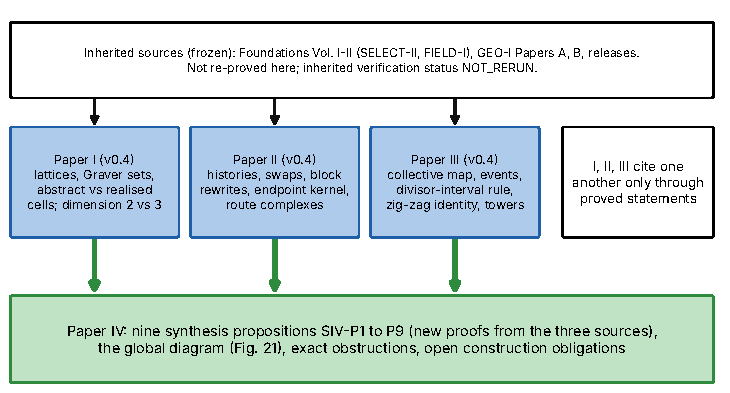
\includegraphics[width=\linewidth]{fig01_architecture.pdf}
\caption{\textbf{Architecture of the programme.} Paper~IV draws only on proved statements of Papers~I--III (v0.4) and on the frozen foundations. \emph{Schematic of inheritance; no mathematical object is drawn.}}\label{fig:arch}\end{figure}

\section{States, histories, occurrence geometry and evolution}\label{sec:objects}
This section fixes the objects, with the exact source of each definition. Notation is collected in Appendix~\ref{app:notation}.

\subsection{Generative states and histories}
\begin{definition}[source: Foundations Vol.~I; \Src{II}{def:select}, \Src{II}{def:history}]
For integers $m,N\ge1$ with $N\mid m$ write $m\xrightarrow{N}T_N(m)=m(N+1)^2/N$. A \emph{history} from the source $m_0$ is a word $w=(N_1,\dots,N_r)$ with $N_i\mid m_{i-1}$, $m_i=T_{N_i}(m_{i-1})$; its \emph{endpoint} is $\Endp(h)=m_r$, its \emph{content} is the multiset $c(h)\in\N^{A}$ of its letters. An adjacent transposition is \emph{legal} if both words are admissible; the \emph{swap graph} on the admissible arrangements of a fixed content has legal transpositions as edges, and its components are the \emph{swap classes}. The \emph{fibre sequence} of $h$ is $F(h)=(D(m_0),\dots,D(m_r))$.
\end{definition}
Since $m_i=m_{i-1}R(N_i)$ with $R(N)=(N+1)^2/N$, the endpoint is $\Endp(h)=m_0\prod_NR(N)^{c_N}$ and depends only on $(m_0,c)$.

\subsection{Collective states}
\begin{definition}[source: Foundations Vol.~II; \Src{III}{def:collective}]
For $x=a/b>0$ in lowest terms, $D(x)=\{d\ge2:d^2\mid a,\ d\equiv1\ (\mathrm{mod}\ b)\}$. If $D(x)\ne\emptyset$ put $L=\lcm D(x)$, $G=\gcd\{d-1\}$ and $C(x)=x+L^2/G$. For an integer $t$ the congruence is vacuous and $D(t)=\{d\ge2:d^2\mid t\}$.
\end{definition}
\begin{lemma}[occurrence monotonicity; \Src{III}{lem:M}]\label{lem:M-cited}
$D(x)\subseteq D(C(x))$. Hence along every orbit $x_n=C^n(x)$ the sets $D_n=D(x_n)$ are non-decreasing.
\end{lemma}

\subsection{Occurrence geometry}
\begin{definition}[the divisor-interval complex; \Src{III}{def:KD}, \Src{III}{thm:R3T1a}, \Src{III}{thm:A5T31}]
For a finite set $D\subset\Z_{\ge2}$ and $u,v\in D$ put $I(u,v)=\{z\in\Z:\gcd(u,v)\mid z\mid\lcm(u,v)\}$. The complex $K(D)$ has vertex set $D$, an edge $\{u,v\}$ iff $I(u,v)\cap(D\cup\{1\})=\{u,v\}$, and higher cells (cubical cells spanned by parallel edges) as in Paper~III. For a state $x$, $\Kmove(x)=K(D(x))$.
\end{definition}
By \Src{III}{thm:R3T1a}, the realised fibre, $\Kmove(x)$, its boundary maps, components and homology are functions of $D(x)$ alone. For an integer $t$, the active primes are those with $p^2\mid t$ and $\Kmove(t)$ is contractible \cite[\Src{III}{thm:B2T1}]{PaperIII}.

\subsection{Lattices and primitive relations}
For a state $x=a/b$ with active primes $p_1,\dots,p_k$ (those $p$ with $p^2\mid a$ and $p\nmid b$) let $\Lambda_b\subseteq\Z^k$ be the lattice of exponent vectors $\alpha$ with $\prod p_i^{\alpha_i}\equiv1\pmod b$, let $F$ be the fibre (its points in the box of admissible exponents, corresponding to $D(x)$) and $\Gr_q(x)$ the region Graver set: the primitive (conformally minimal) lattice vectors in the box. These are the objects of Paper~I; their transport under change of lattice is governed by \Src{I}{thm:P2T1} and \Src{I}{thm:P2T2}, abstract cells by \Src{I}{thm:cell-transport}, and the failure of laws one might expect by \Src{I}{thm:laws}.

\subsection{Factorization}
\begin{lemma}[factorization criterion]\label{lem:factor}
Let $\pi:X\to Y$ be surjective and $f:X\to Z$. Then $f=g\circ\pi$ for some $g$ iff $f$ is constant on every fibre of $\pi$; $g$ is then unique. If two points $x,x'$ have $\pi(x)=\pi(x')$ and $f(x)\ne f(x')$, no such $g$ exists.
\end{lemma}
\begin{proof}Define $g(y)=f(x)$ for any $x\in\pi^{-1}(y)$; well-definedness is constancy on fibres. The last statement is the contrapositive.\end{proof}
Throughout, an \emph{obstruction} to a factorization is a pair $x,x'$ as in the last sentence together with a proof that $\pi(x)=\pi(x')$ and $f(x)\neq f(x')$; its \emph{domain} is the set on which $\pi$ is taken (a fixed source, or all integers) and is stated each time.


\noindent\Cref{fig:states} shows arithmetic states and the objects attached to them.

\begin{figure}[t]\centering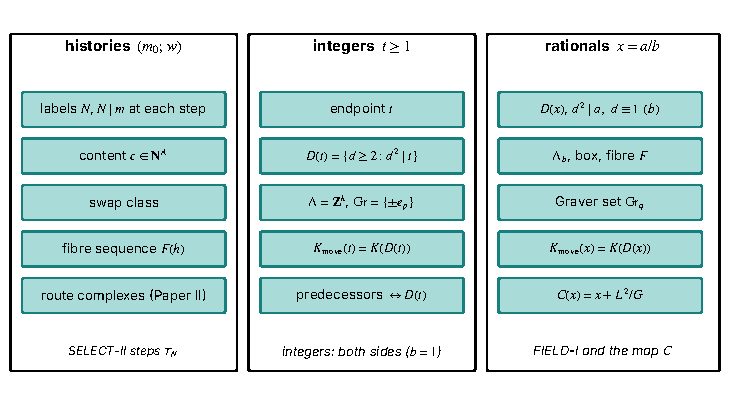
\includegraphics[width=\linewidth]{fig02_states_objects.pdf}
\caption{\textbf{Arithmetic states and the objects attached to them.} Three domains with their native constructions. Integers are the overlap: an integer is both an endpoint of histories and a collective state with denominator $1$. \emph{Schematic of domains.}}\label{fig:states}\end{figure}

\section{Numerical projection and generative information}\label{sec:numerical}
Fix a source $m_0$. Let $\Hist(m_0)$ be the set of histories from $m_0$. Three projections are in play:
\[
\Hist(m_0)\xrightarrow{\ \pi_1\ }\mathrm{Cls}(m_0)\xrightarrow{\ \pi_2\ }\mathrm{Cont}(m_0)\xrightarrow{\ \pi_3\ }\mathrm{End}(m_0)\subseteq\Z,
\]
\[
h\mapsto[h]\mapsto c(h)\mapsto m_0\prod_NR(N)^{c_N}=\Endp(h).
\]
Here $\mathrm{Cls}(m_0)$ is the set of swap classes (all words in a class have the same content, since legal swaps are transpositions) and $\mathrm{Cont}(m_0)$ the set of contents of admissible histories, and $\mathrm{End}(m_0)=\{\Endp(h)\}$ the set of reachable endpoints; the codomain of $\pi_3$ is $\mathrm{End}(m_0)$, not all of $\Z$, so that $\pi_1,\pi_2,\pi_3$ are surjections. For a finite alphabet $A$ write $\mathrm{Cont}_A(m_0)\subseteq\mathrm{Cont}(m_0)$ for the admissible contents supported on $A$, $\mathrm{End}_A(m_0)$ for the endpoints of histories over $A$, and $\pi_{3,A}:\mathrm{Cont}_A(m_0)\to\mathrm{End}_A(m_0)$ for the restriction of $\pi_3$; the matrix $V_A$ acts on $\Z^A$ and so only on contents supported on $A$.

\subsection{Cited ingredients}
\begin{theorem}[kernel condition; \Src{II}{thm:kernel}]\label{thm:kernel-cited}
Let $A$ be a finite alphabet, $\mathcal P$ the primes dividing some $N$ or $N+1$, $N\in A$, and $V_A=(\Delta_p(N))_{p\in\mathcal P,N\in A}$ with $\Delta_p(N)=2v_p(N+1)-v_p(N)$. Two histories over $A$ from the same source have the same endpoint iff $V_A(c-c')=0$.
\end{theorem}
\begin{theorem}[faithfulness; \Src{II}{thm:faith}]\label{thm:faith-cited}
For a fixed source the fibre sequence $F(h)$ determines the history $h$. A legal swap changes exactly one entry of $F(h)$.
\end{theorem}
\begin{theorem}[classification for $\{2,3,14\}$; \Src{II}{thm:2314}]\label{thm:2314-cited}
The number $\nu(m)$ of swap classes of $\{2,3,14\}$ at the source $m$ is $0$ if neither $14$ nor $21$ divides $m$, $2$ if $14\mid m$ and $\gcd(m/14,6)=1$, and $1$ otherwise.
\end{theorem}

\subsection{The proposition}
\begin{proposition}[\SIV{1}: endpoint projection and retained information]\label{prop:P1}\status{new, proved}
Let $m_0\ge1$.
\begin{enumerate}[label=(\alph*),itemsep=1pt]
\item \emph{Factorization.} The maps $\pi_1,\pi_2,\pi_3$ are well defined and $\Endp=\pi_3\pi_2\pi_1$. Thus the endpoint is a function of the content, and of the swap class, of the history; and a numerical invariant of the endpoint is a function of $(m_0,\text{content})$.
\item \emph{What the endpoint retains.} For histories over a common alphabet $A$ the endpoint determines exactly the vector $V_Ac=(v_p(t)-v_p(m_0))_{p\in\mathcal P}$, and conversely this vector determines the endpoint. The fibre of $\pi_{3,A}$ over a reachable endpoint $t=\Endp(h)$ with $h$ over $A$ is $\pi_{3,A}^{-1}(t)=\mathrm{Cont}_A(m_0)\cap\bigl(c(h)+\ker_{\Z}V_A\bigr)$: the coset must be intersected with the set of \emph{admissible} contents from $m_0$ supported on $A$, not merely with $\N^A$. (Histories using letters outside $A$ and ending at $t$ are in the fibre of $\pi_3$ but not of $\pi_{3,A}$; they are compared by enlarging $A$.) Example: $m_0=1$, $A=\{1,2,3\}$, $c=(7,0,0)$ and $c'=(0,2,4)$ have $R(1)^7=R(2)^2R(3)^4=16384$, so $c-c'\in\ker_\Z V_A$ and $c'\in\N^A$, yet $c'\notin\mathrm{Cont}_A(1)$ because neither label $2$ nor label $3$ can be applied first.
\item \emph{Each projection is non-injective.} (i) $\pi_3$: at $m_0=32$ the histories $(2,2,2,2)$ and $(1,8,8)$ are admissible with the same endpoint $13122$ and different content and length. (ii) $\pi_2$: at $m_0=14$ the contents of $(14,3,2)$ and $(2,3,14)$ coincide, both end at $5400$, but they lie in different swap classes. (iii) $\pi_1$: from $m_0=1$ the two histories $(1,2,1),(1,1,2)$ to $72$ lie in one class.
\item \emph{Invariants.} Functions of $(m_0,\Endp(h))$ factor through $\pi_3\pi_2\pi_1$ (this includes, for fixed $m_0$, the number $H(m_0,t)$ of histories from $m_0$ to $t$, which depends only on $t$); the length $r$ of $h$, the content and the swap class do not factor through $\pi_3$ on any set of sources containing the witnesses in (c). The number of histories to $t$ is a function of $t$ but does \emph{not} factor through the occurrence set $D(t)$ (\cref{prop:P5}).
\end{enumerate}
\end{proposition}
\begin{proof}
(a) A legal swap exchanges two adjacent letters, so the content is invariant; hence $\pi_2$ is defined on classes. The product formula $\Endp(h)=m_0\prod R(N_i)$ gives $\pi_3$. (b) is \cref{thm:kernel-cited} together with the identity $v_p(\Endp(h))-v_p(m_0)=\sum_N c_N\Delta_p(N)=(V_Ac)_p$, which follows from $v_p(R(N))=2v_p(N+1)-v_p(N)$. For the fibre: a content $c'\in\mathrm{Cont}_A(m_0)$ has the endpoint $t$ iff $V_A(c'-c)=0$, i.e.\ iff $c'\in c+\ker_\Z V_A$; the example has $V_A(c-c')=0$ by $R(1)^7=4^7=16384=(9/2)^2\cdot(16/3)^4$, and $c'$ is inadmissible from $1$ since admissibility of a first letter $N$ requires $N\mid m_0=1$. (c)(i): $T_2$ applied to $32,144,648,2916$ (all even) gives $144,648,2916,13122$; and $32\to128\to1296\to13122$ by $T_1,T_8,T_8$ with $8\mid128$ and $8\mid1296$. Lengths are $4$ and $3$. (ii): $14\to225\to1200\to5400$ by $T_{14},T_3,T_2$ with $3\mid225$, $2\mid1200$, and $14\to63\to336\to5400$ by $T_2,T_3,T_{14}$ with $3\mid63$, $14\mid336$. By \cref{thm:2314-cited} with $m=14$ ($14\mid14$, $\gcd(1,6)=1$) there are two classes; the only admissible arrangements are these two. (iii): $72=1\cdot4\cdot\tfrac92\cdot4$ and the two words differ by one legal adjacent transposition. (d) The first sentence follows from (a) and \cref{lem:factor}; the non-factorization of $r$, content and class through $\pi_3$ is the witnesses of (c). For the last sentence: the count $H(m_0,t)$ is by definition constant on the fibres of $\pi_3$, and its failure to factor through $D(t)$ is the witness pairs of \cref{prop:P5}.
\end{proof}
\begin{remark}
\cref{prop:P1}(b) is the precise sense in which the endpoint is a \emph{valuation-displacement}: it forgets how that displacement was composed from letters. The identity $\sum_Nc_N\Delta_p(N)=(V_Ac)_p$ is the same arithmetic that organises the gain--loss accounting of \Src{III}{thm:B2T3}.
\end{remark}

\noindent\Cref{fig:endpoint} shows endpoint projection and its fibres.

\begin{figure}[t]\centering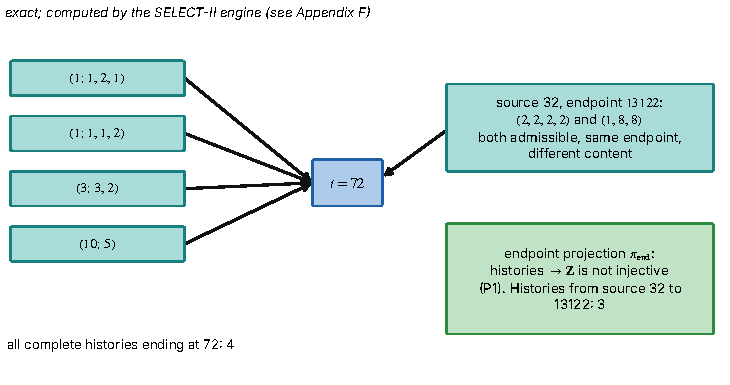
\includegraphics[width=\linewidth]{fig03_endpoint_fibres.pdf}
\caption{\textbf{Endpoint projection and its fibres} ($\pi_3$ of \cref{prop:P1}). Left: the four complete histories that end at $72$, from sources $1,1,3,10$. Right: two histories from source $32$ with the same endpoint and different content. \emph{Exact; computed by the history engine (Appendix~\ref{app:finite}).}}\label{fig:endpoint}\end{figure}

\noindent\Cref{fig:anc72} shows four histories reaching $72$ and their structural records.

\begin{figure}[t]\centering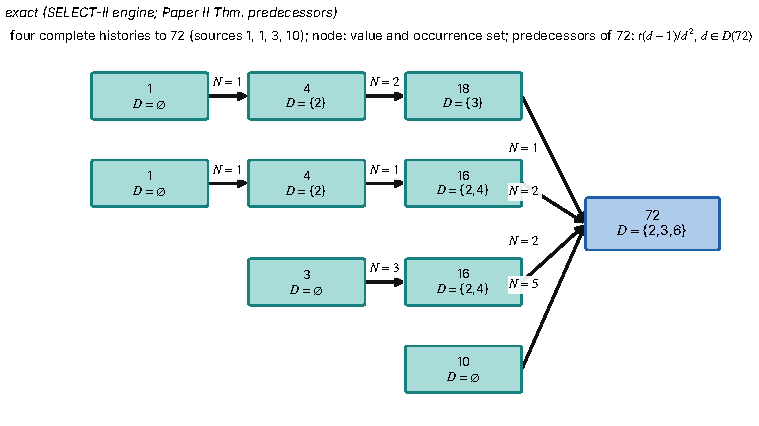
\includegraphics[width=\linewidth]{fig04_ancestry_72.pdf}
\caption{\textbf{Four histories reaching $72$ and their structural records.} Each node shows an integer and its occurrence set $D$; arrows are SELECT-II steps labelled by $N$. The four paths have different fibre sequences $F(h)$, although they share the endpoint $72$ and the same terminal data $D(72)=\{2,3,6\}$ (\Src{II}{thm:predecessors}, \Src{II}{thm:faith}). \emph{Exact.}}\label{fig:anc72}\end{figure}

\noindent\Cref{fig:kernel} shows same endpoint, different label content.

\begin{figure}[t]\centering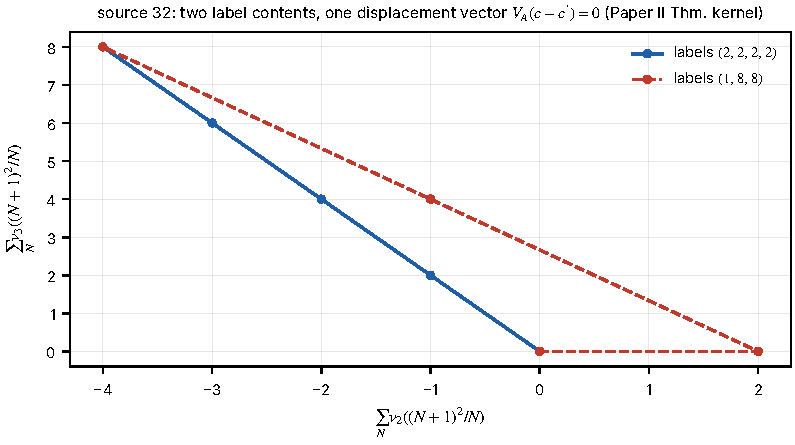
\includegraphics[width=0.85\linewidth]{fig05_kernel_ambiguity.pdf}
\caption{\textbf{Same endpoint, different label content.} Cumulative displacement of $(v_2,v_3)$ of the running value for the label words $(2,2,2,2)$ and $(1,8,8)$ from source $32$: both paths end at $V_A c=V_Ac'$ (\cref{thm:kernel-cited}). \emph{Exact.}}\label{fig:kernel}\end{figure}

\section{Occurrence projection and dormant arithmetic structure}\label{sec:occurrence}
The second projection sends a state to its occurrence set. For integers it has a direct generative meaning.

\begin{proposition}[\SIV{2}: occurrence projection and primitive-relation information]\label{prop:P2}\status{new, proved; (b),(c) cited}
\begin{enumerate}[label=(\alph*),itemsep=1pt]
\item \emph{Occurrences are incoming steps.} For an integer $t\ge1$ the map $d\mapsto(N,m)=\bigl(d-1,\ t(d-1)/d^2\bigr)$ is a bijection from $D(t)$ onto the set of generative steps $m\xrightarrow{N}t$. Consequently $|D(t)|$ is the in-degree of $t$, and for every $m_0$ the number $H(m_0,t)$ of histories from $m_0$ to $t$ satisfies $H(m_0,t)=\sum_{d\in D(t)}H\bigl(m_0,\ t(d-1)/d^2\bigr)$ (with $H(m_0,m_0)=1$ and the convention that terms with $t(d-1)/d^2<m_0$ vanish). Moreover $N+1\in D(T_N(m))$ for every admissible step.
\item \emph{Factorization.} The realised fibre, $\Kmove(x)$ and all its derived data factor through $x\mapsto D(x)$; for integer $t$ the whole record is a function of $\max D(t)$ (\Src{III}{thm:R3T1a}, \Src{III}{thm:B2T1}).
\item \emph{Obstruction.} The primitive relation system does not factor through $D$: for primes $r\ge13$, $r\equiv5\pmod8$, the states $x_r=25r^2/(5r-1)$ and $y_r=25r^2/8$ have $D(x_r)=D(y_r)=\{5r\}$ and the same active primes and box, but $|\Gr(x_r)|=2$ and $|\Gr(y_r)|=4$ (\Src{III}{thm:R3T1}(i)).
\end{enumerate}
\end{proposition}
\begin{proof}
(a) If $m\xrightarrow{N}t$ then $t=m(N+1)^2/N$ with $N\mid m$; we have $tN=m(N+1)^2$, so $(N+1)^2\mid tN$, and $\gcd(N,N+1)=1$ gives $(N+1)^2\mid t$, i.e.\ $d=N+1\in D(t)$ (here $d\ge2$), and $m=tN/(N+1)^2=t(d-1)/d^2$. Conversely if $d\in D(t)$ put $N=d-1$ and $m=t(d-1)/d^2$; then $m\in\Z$ because $d^2\mid t$, $N\mid m$ because $m=(t/d^2)N$, and $T_N(m)=m(N+1)^2/N=t$. The two assignments are inverse. A history to $t$ is a history to the predecessor $m$ followed by the step to $t$, which gives the recursion. For the last statement $(N+1)^2\mid m(N+1)^2/N=T_N(m)$ because $N\mid m$ makes $m/N$ an integer.
(b) and (c) are the cited theorems; for (c) we recomputed $D(x_{13})=D(y_{13})=\{65\}$ (Appendix~\ref{app:finite}).
\end{proof}
\begin{corollary}\label{cor:P2}
The occurrence set of an integer is the branching set of its ancestry: histories to $t$ are sequences of choices of elements of $D$ along the way. Hence the invariant counting histories depends on $t$ through the recursion above, not through $D(t)$ alone (compare \cref{prop:P5}).
\end{corollary}
\paragraph{Information chain.} Combining \cref{prop:P2} with \cref{prop:P1}: the chain $\mathrm{Hist}\to\mathrm{Cls}\to\mathrm{Cont}\to\Z\to\{D\}\to\{\Kmove\}\to\{\beta\}$ consists of surjections, each a factorization of the next by \cref{lem:factor}; the first three arrows lose information on every set containing the witnesses of \cref{prop:P1}; the fourth, $t\mapsto D(t)$, is non-injective (all $t$ with the same square-divisor set, \cref{prop:P5}); and $D\mapsto\Gr$ does not exist at all (\cref{prop:P2}(c)). \cref{fig:fact} shows the chain with the status of each arrow.
\begin{figure}[t]\centering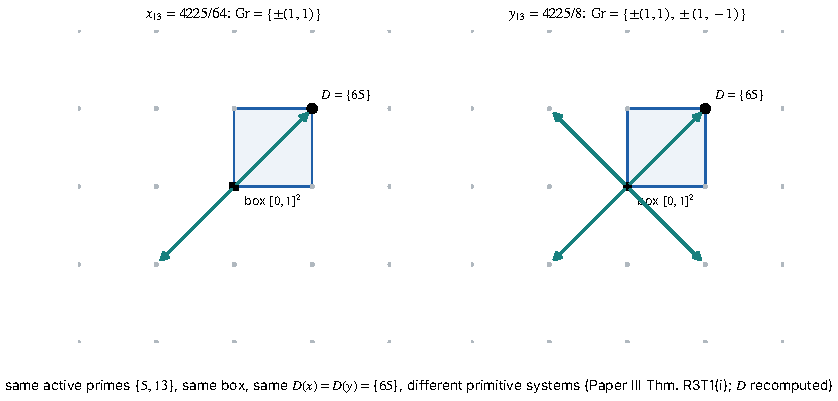
\includegraphics[width=\linewidth]{fig06_equalD_diffGr.pdf}
\caption{\textbf{Occurrence projection and dormant relations.} The states $x_{13}=4225/64$ and $y_{13}=4225/8$ have the same occurrence set $\{65\}$, the same active primes $\{5,13\}$ and the same box $[0,1]^2$, but the primitive systems differ: the extra pair $\pm(1,-1)$ is a primitive relation of $y_{13}$ that is not realised at $x_{13}$. \emph{Exact data of \Src{III}{thm:R3T1}(i) with $r=13$; $D$ recomputed; the lattice pictures are schematic.}}\label{fig:equalD}\end{figure}

\section{Geometric realization and dimensional transport}\label{sec:realization}
\subsection{Three tiers of relation}
For a state $x$ there are three nested layers of arithmetic relation: the relations of the lattice $\Lambda_b$ (arithmetic availability), the primitive relations $\Gr_q(x)$, and the \emph{realised moves}, the edges of $\Kmove(x)$, which are pairs of occurrences present in $D(x)$. \cref{fig:possible} depicts the layers; what is proved about each is collected in \cref{prop:P3}.

\subsection{An abstract minimality principle}
\begin{definition}
Let $(P,\prec)$ be a strict partial order and $X\subseteq P$. Put $\min_\prec X=\{g\in X:\ \nexists\,x\in X,\ x\prec g\}$.
\end{definition}
\begin{lemma}[monotone minimality]\label{lem:minimal}
If $X\subseteq X'\subseteq P$ and $g\in\min X$, then $g\in\min X'$ iff no element of $X'\setminus X$ lies below $g$. In particular, if $X_0\subseteq X_1\subseteq\cdots$ and $g\in\min X_{n_0}$, the set $\{n\ge n_0:g\in\min X_n\}$ is an initial segment of $\{n_0,n_0+1,\dots\}$.
\end{lemma}
\begin{proof}
$g\in X'$. An element of $X'$ below $g$ lies either in $X$, impossible by minimality in $X$, or in $X'\setminus X$. For the second claim, if $g\notin\min X_n$ then some $z\in X_n$, $z\prec g$, which stays in $X_{n'}$ for $n'\ge n$.
\end{proof}
\noindent Two instances occur in the sources. (I) Paper~I: $P$ is a lattice with the conformal order $\sqsubseteq$ on integer vectors, $X=\Lambda\setminus\{0\}$, $\min X=\Gr(\Lambda)$; \Src{I}{thm:P2T2} says $g\in\Gr_q(\Lambda')$ iff $g\in\Lambda'$ and no $v\in\Lambda'\setminus\{0,g\}$ satisfies $v\sqsubseteq g$, which is the lemma for $X=\Lambda$, $X'=\Lambda'$ when $\Lambda\subseteq\Lambda'$. (II) Paper~III: for a fixed pair $e=\{u,v\}$ with $\gcd(u,v)>1$ let $P=\{e\}\cup\bigl(I(u,v)\setminus\{u,v\}\bigr)$ with $z\prec e$ for every $z\ne e$, and $X_n=\{e\}\cup(D_n\cap I(u,v)\setminus\{u,v\})$. Then $e\in\min X_n$ iff $D_n\cap(I(u,v)\setminus\{u,v\})=\emptyset$, which by \Src{III}{thm:A5T31} is the condition for $e$ to be an edge once $u,v\in D_n$. The two instances share only the logical shape of the criterion; the ambient sets are different.

\begin{proposition}[\SIV{3}: arithmetic availability versus geometric realization]\label{prop:P3}\status{new, proved; (c),(d) cited}
Let $x_n=C^n(x)$ and $D_n=D(x_n)$.
\begin{enumerate}[label=(\alph*),itemsep=1pt]
\item \emph{Availability of vertices is monotone.} If $u,v\in D_n$ then $u,v\in D_{n'}$ for all $n'\ge n$.
\item \emph{Realisation windows.} For $u,v\in\bigcup_nD_n$, $u\ne v$, let $a(u)=\min\{n:u\in D_n\}$ and $p(u,v)=\min\{n:\ D_n\cap(I(u,v)\setminus\{u,v\})\ne\emptyset\}$ (the first time the interval is pierced by an occurrence; $\infty$ if never; note $1\in I(u,v)$ only if $\gcd(u,v)=1$). Then $\{u,v\}$ is an edge of $\Kmove(x_n)$ iff $\max(a(u),a(v))\le n<p(u,v)$ and, when $\gcd(u,v)=1$, never. In particular the set of times at which a fixed pair is a realised move is an interval of consecutive integers (possibly empty): an edge that disappears never returns.
\item \emph{Availability does not imply a primitive relation is realised.} For $k\ge2$ and the family of \Src{III}{thm:A4T1} the relation $e_i-e_j$ is primitive at $x=P^2/\ell$ (with $D(x)=\{P\}$) and has no pair of fibre points, hence is not realised; it is realised at $y=(Pq)^2/\ell$.
\item \emph{Occurrence inclusion does not control primitive persistence} (\Src{I}{thm:laws}, law L1), whereas persistence of a realised move is controlled by $D$ as in (b).
\end{enumerate}
\end{proposition}
\begin{proof}
(a) is \cref{lem:M-cited}. (b) By \cref{thm:A5T31-cited} below, $\{u,v\}$ is an edge of $\Kmove(x_n)$ iff $u,v\in D_n$ and $I(u,v)\cap(D_n\cup\{1\})=\{u,v\}$. If $\gcd(u,v)=1$ then $1\in I(u,v)\setminus\{u,v\}$ (as $u,v\ge2$), so there is never an edge. If $\gcd(u,v)>1$ then $1\notin I(u,v)$ and the condition is $u,v\in D_n$ and $D_n\cap(I(u,v)\setminus\{u,v\})=\emptyset$, i.e.\ $n\ge\max(a(u),a(v))$ and $n<p(u,v)$ by monotonicity of $D_n$. (c), (d) are cited.
\end{proof}
\begin{theorem}[divisor-interval rule; \Src{III}{thm:A5T31}]\label{thm:A5T31-cited}
Distinct $u,v\in D(x)$ are joined by an edge of $\Kmove(x)$ iff $I(u,v)\cap(D\cup\{1\})=\{u,v\}$.
\end{theorem}
\begin{corollary}[answer to S4, structural part]\label{cor:S4}
The persistence criterion for primitive relations in Paper~I (\Src{I}{thm:P2T2}) and the edge-loss criterion in Paper~III (\Src{III}{thm:A5T31}) are instances of \cref{lem:minimal}, with the ambient orders the conformal order on a lattice and the divisor-interval order on $D$ respectively. An implication from one to the other would need an identification of the two ambient sets; this is open (O7) and is \emph{not} claimed.
\end{corollary}
\begin{figure}[t]\centering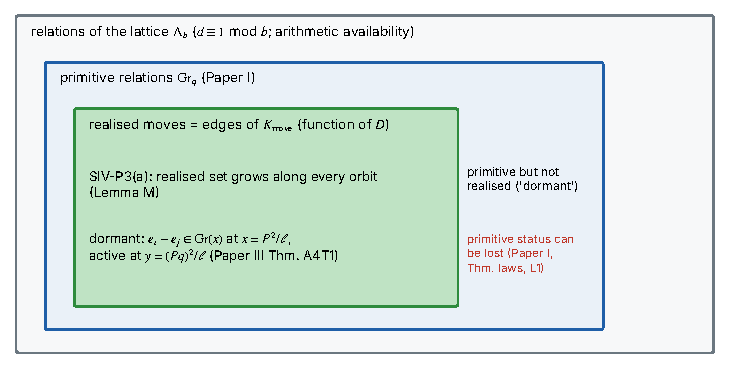
\includegraphics[width=\linewidth]{fig07_possible_vs_realised.pdf}
\caption{\textbf{Arithmetic possibility versus geometric realization.} The relation lattice contains the primitive relations, which contain what is realised as moves of $\Kmove$; the realised set is a function of $D$ and grows along orbits (\cref{prop:P3}(a)), primitive status can be lost. \emph{Schematic of containments; cited exact examples are named.}}\label{fig:possible}\end{figure}

\subsection{The dimensional boundary of transport}
Paper~I proves that for lattices $\Lambda\subseteq\Lambda'$ in rank two the realised union of cells is monotone (\Src{I}{thm:planar}) and that this fails in rank three without a free coordinate (\Src{I}{thm:C1}), with a corner-cube criterion (\Src{I}{thm:corner}) and a slab description when a free coordinate exists (\Src{I}{thm:slab-i}). These statements are about lattice transport, and the relation to occurrence geometry is through \cref{prop:P3}(c),(d): occurrence inclusion is not a lattice inclusion. Finally, abstract loss of a cell does not mean loss from the realised union (\Src{I}{prop:topology}, specimen $21^8/5\to21^8/4$: abstract Betti numbers $(1,5,0)\to(1,2,6)$, realised $(1,2,0)\to(1,0,0)$).

\noindent\Cref{fig:dim} shows planar preservation and three-dimensional failure.

\begin{figure}[t]\centering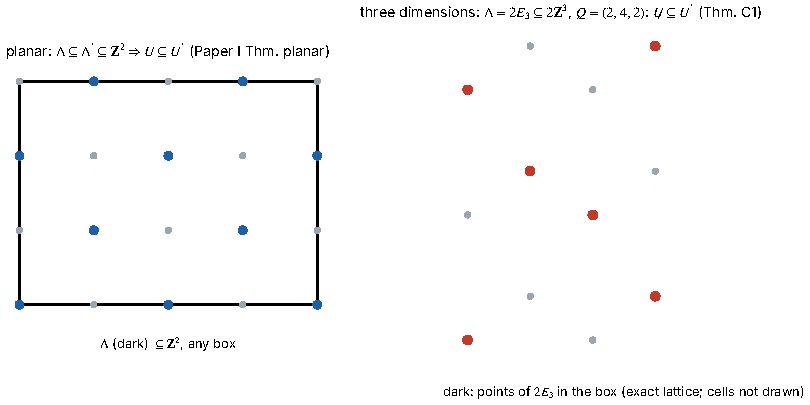
\includegraphics[width=\linewidth]{fig08_planar_vs_3d.pdf}
\caption{\textbf{Planar preservation and three-dimensional failure.} Left: \Src{I}{thm:planar}. Right: \Src{I}{thm:C1} with $\Lambda=2E_3\subseteq2\mathbf{Z}^3$ and box $(2,4,2)$. \emph{Theorem-level schematic: lattice points are exact, cells are not drawn.}}\label{fig:dim}\end{figure}

\noindent\Cref{fig:abs} shows abstract cell loss versus realised geometric containment.

\begin{figure}[t]\centering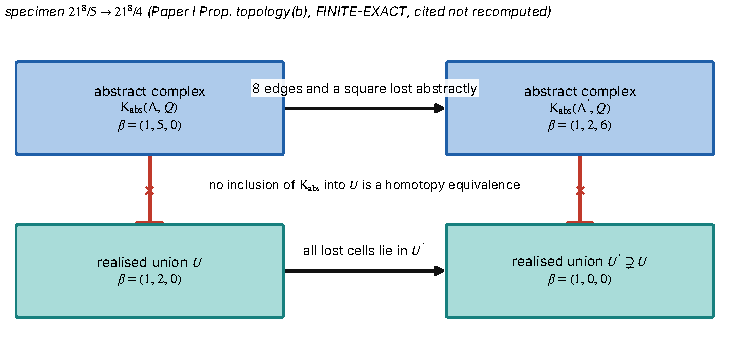
\includegraphics[width=\linewidth]{fig09_abstract_vs_realised.pdf}
\caption{\textbf{Abstract cell loss versus realised geometric containment.} For the planar specimen of \Src{I}{prop:topology}(b) the abstract complex loses cells while the realised union grows. \emph{Finite-exact values quoted from Paper~I, not recomputed.}}\label{fig:abs}\end{figure}

\section{Arithmetic constraints and history topology}\label{sec:history}
\subsection{Local guards and global classes}
A single legal swap is a local arithmetic condition: for adjacent letters $N,N'$ at a state $m$, both $N\mid m,\ N'\mid mR(N)$ and $N'\mid m,\ N\mid mR(N')$ must hold. Whether the \emph{global} space of arrangements of a content is connected depends on how these conditions interact along all positions. The sharpest exact statement available is the classification of $\{2,3,14\}$ (\cref{thm:2314-cited}), together with a general separation principle.
\begin{theorem}[a separator of swap classes; \Src{II}{thm:R3T3}]\label{thm:R3T3-cited}
Let $A$ be a set of distinct labels with $A\cap\{1,2,4\}=\emptyset$, the source $4$ and the content $\{2,4\}\cup A$. For an admissible arrangement $w$ let $I(w)=1$ if $2$ precedes $4$ and $0$ otherwise. Then $I$ is constant on swap classes; consequently the number of classes is at least the number of values of $I$ that occur.
\end{theorem}
\begin{theorem}[route cubes; \Src{II}{thm:cube}]\label{thm:cube-cited}
For every $r\ge1$ the complete histories ending at $72^r$ contain an $r$-cube: from source $1$, the prefix $1^r$ followed by $r$ blocks, each independently $(1,2)$ or $(2,1)$.
\end{theorem}
\begin{proposition}[\SIV{4}: arithmetic constraints and global history connectivity]\label{prop:P4}\status{new, proved from cited theorems; finite check}
\begin{enumerate}[label=(\alph*),itemsep=1pt]
\item \emph{Swap-invariant separators.} If $\phi$ is a function on the admissible arrangements of a content that is invariant under legal swaps, the number of swap classes is at least $|\phi(\text{arrangements})|$. (An obstruction to connectivity is thus certified by one invariant.)
\item \emph{Connectivity is not monotone in the source.} For $\{2,3,14\}$: $\nu(7)=0$, $\nu(14)=2$, $\nu(28)=1$, $\nu(70)=2$. Hence the class count increases from $7$ to $14$, decreases from $14$ to $28$, and is not a function of divisibility order.
\item \emph{Connectivity is not a function of content and displacement alone.} The content $\{2,3,14\}$ gives $\nu=2$ at $m=14$ and $\nu=1$ at $m=28$; the displacement vector $V_Ac$ is the same in both cases (it depends on the content only). Hence content together with valuation displacement, without the source, does not determine the class count across different sources. (This compares two sources and is therefore not a statement about the information retained by the endpoint projection $\pi_3$ of one fixed source; for that see \cref{prop:P1}(b) and \cref{prop:P5}.)
\item \emph{Local freedom with global rigidity.} The 2-cube of histories $1\to72^2$ consists of four histories joined in a 4-cycle of legal swaps; it is a subgraph of the swap graph of all $16$ histories $1\to5184$ (exhaustive count).
\end{enumerate}
\end{proposition}
\begin{proof}
(a) Constancy on classes plus distinct values give distinct classes. (b) Substituting into \cref{thm:2314-cited}: $m=7$: neither $14$ nor $21$ divides $7$, so $\nu=0$; $m=14$: $14\mid14$, $\gcd(1,6)=1$, so $\nu=2$; $m=28$: $14\mid28$, $\gcd(2,6)=2$, so $\nu=1$; $m=70$: $\gcd(5,6)=1$, $\nu=2$. Since $7\mid14\mid28$ and $14\mid70$ the pattern up, down, up shows non-monotonicity in the divisibility order. (A direct check of the formula on all sources $1\le m<1500$ found no deviation; Appendix~\ref{app:finite}.) (c) is read off from (b): $\nu(14)\ne\nu(28)$ with the same content, hence the same $V_Ac$, at the two different sources $14$ and $28$. (d) is \cref{thm:cube-cited} for $r=2$ together with the exhaustive history count of Appendix~\ref{app:finite}; adjacent words in the cube differ by one transposition of a block, which is legal since both orders are histories.
\end{proof}

\noindent\Cref{fig:swap} shows local swaps and globally disconnected history classes.

\begin{figure}[t]\centering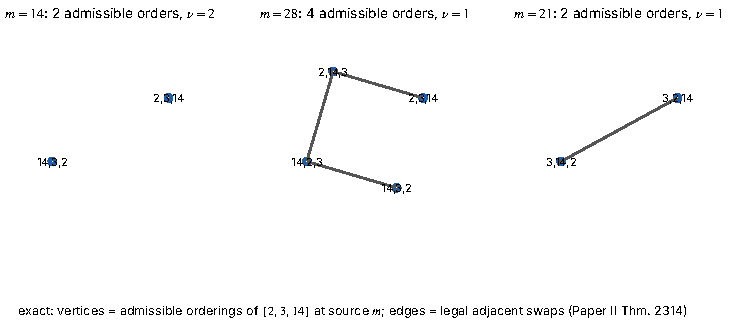
\includegraphics[width=\linewidth]{fig10_swap_components.pdf}
\caption{\textbf{Local swaps and globally disconnected history classes.} Swap graphs of the admissible orders of $\{2,3,14\}$ at the sources $14$, $28$, $21$ (\Src{II}{thm:2314}); the number of components is $\nu=2,1,1$. \emph{Exact; computed.}}\label{fig:swap}\end{figure}

\subsection{Cubes and homology}
A combinatorial cube of legal swaps is contractible once filled; the homology of the route complex of all histories to an integer records more. Paper~II proves that route complexes can have nontrivial higher-dimensional homology in suitable families (see \Src{II}{thm:sphere}, \Src{II}{thm:dual}); we use only the logical point that \emph{the presence of cubes does not decide the homology}, which is why the history side requires its own computations and cannot be read from $K(D(t))$ (\cref{prop:P5}).

\noindent\Cref{fig:loop} shows a history loop and a higher-dimensional void.

\begin{figure}[t]\centering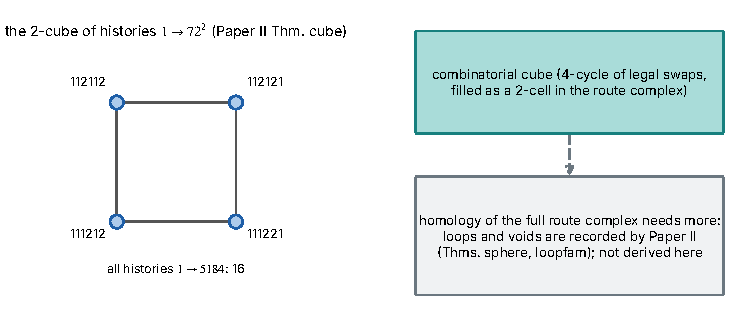
\includegraphics[width=\linewidth]{fig11_loop_void.pdf}
\caption{\textbf{A history loop and a higher-dimensional void.} Left: the 2-cube of histories $1\to5184$ (exact words). Right: what is and is not claimed; the homology of full route complexes is recorded in Paper~II. \emph{Left exact, right schematic.}}\label{fig:loop}\end{figure}

\section{Endpoint geometry versus global ancestry}\label{sec:endpoint}
For an integer $t$ the endpoint geometry is $K(D(t))$ together with everything determined by $D(t)$ (\cref{prop:P2}). The ancestry of $t$ is its set of complete histories, their classes and their complexes. \cref{prop:P5} separates them.
\begin{proposition}[\SIV{5}: limits of endpoint geometry as a history invariant]\label{prop:P5}\status{new, proved by exhaustive recursion; finite-exact witnesses}
\begin{enumerate}[label=(\alph*),itemsep=1pt]
\item \emph{Obstruction.} $D(900)=D(9000)=\{2,3,5,6,10,15,30\}$, hence $K(D(900))=K(D(9000))$ and all of the data of \cref{prop:P2}(b) coincide, but from the source $4$ there are $2$ histories forming $1$ swap class to $900$ and $4$ histories forming $2$ swap classes to $9000$. Likewise $D(288)=D(4320)$ with $(3\text{ histories},1\text{ class})$ and $(3,2)$ from source $4$.
\item \emph{Consequence.} Neither the number of histories, nor the number of swap classes, nor the isomorphism type of the swap graph of $\Hist(4,t)$ factors through $t\mapsto D(t)$ (\cref{lem:factor}); \emph{a fortiori} none of them factors through $K(D(t))$ or its Betti numbers.
\item \emph{Frequency (finite-exact).} Let $E$ range over the integers $16\le E\le120000$ that are not squarefree and are reachable from the source $4$. They realise $238$ distinct occurrence sets $D(E)$; $166$ of these sets are shared by several $E$, and for $106$ of them the number of swap classes is not constant (for $158$ the number of histories is not constant). This is a finite census and is not extrapolated.
\item \emph{What would suffice.} The fibre sequence $F(h)$ determines the history (\cref{thm:faith-cited}); so the occurrence sets \emph{along the path} reconstruct ancestry, but the occurrence set of the endpoint does not (S2, S3).
\end{enumerate}
\end{proposition}
\begin{proof}
(a) By \cref{prop:P2}(a) the history counts satisfy $H(4,t)=\sum_{d\in D(t)}H(4,t(d-1)/d^2)$; the recursion terminates because predecessors decrease. We evaluated it exactly for $900$ and $9000$ (and for $288,4320$); the $2$ histories to $900$ and the $4$ to $9000$ are listed in Appendix~\ref{app:obstructions}, and the swap classes are computed by union--find over legal adjacent transpositions of those words. $D(900)=D(9000)$ is read off from $900=2^23^25^2$ and $9000=2^33^25^3$: in both, $d^2$ divides the number iff $d\mid30$. (b) is \cref{lem:factor}. (c) is a recorded exhaustive computation (Appendix~\ref{app:finite}). (d) is \cref{thm:faith-cited}.
\end{proof}

\noindent\Cref{fig:endhist} shows endpoint move complex versus history complex.

\begin{figure}[t]\centering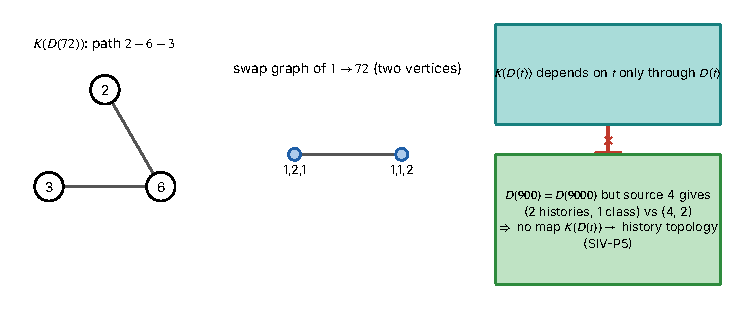
\includegraphics[width=\linewidth]{fig12_endpoint_vs_history.pdf}
\caption{\textbf{Endpoint move complex versus history complex.} Left: $K(D(72))$ is the path $2-6-3$. Middle: the swap graph of the histories $1\to72$ has two vertices. Right: the obstruction \SIV{5}. \emph{Exact; the right panel is schematic.}}\label{fig:endhist}\end{figure}

\section{Structural changes during collective evolution}\label{sec:evolution}
Let $x_0$ be a state with $D(x_0)\ne\emptyset$ and $x_n=C^n(x_0)$, $D_n=D(x_n)$, $K_n=K(D_n)$. By \cref{lem:M-cited} $D_0\subseteq D_1\subseteq\cdots$, but the complexes $K_n$ are not nested: new occurrences pierce intervals and kill edges. The question is which structural features persist.

\subsection{Connectivity is governed by prime supports}
\begin{lemma}[component rule]\label{lem:comp}
For a finite $D\subset\Z_{\ge2}$ the components of $K(D)$ are the classes of the equivalence relation on $D$ generated by $u\approx v\iff\gcd(u,v)>1$. Equivalently $\beta_0(K(D))$ is the number of connected components of the bipartite graph between $D$ and the set of primes dividing elements of $D$ (with $d\sim p$ iff $p\mid d$).
\end{lemma}
The proof is in Appendix~\ref{app:proofs}; it uses only the interval criterion \cref{thm:A5T31-cited}: a coprime pair is never an edge because $1\in I(u,v)$, and a pair with $\gcd>1$ is joined by a path obtained by induction on $|I(u,v)|$. The lemma was also checked on $3000$ random sets (Appendix~\ref{app:finite}).
\begin{proposition}[\SIV{6}: hierarchy of structural persistence under evolution]\label{prop:P6}\status{new, proved; (d) uses cited census}
Along an orbit:
\begin{enumerate}[label=(\alph*),itemsep=1pt]
\item \emph{Vertices} persist: $D_n\subseteq D_{n+1}$.
\item \emph{Connectivity} persists: if $u,v\in D_n$ lie in one component of $K_n$ they lie in one component of $K_{n+1}$. Hence each component of $K_n$ is contained in a unique component of $K_{n+1}$, and $\beta_0$ changes only by merging old components and by adding components consisting of new vertices; a component never splits.
\item \emph{Edges} do not persist in general: a pair $\{u,v\}$ is an edge during exactly the interval $[\max(a(u),a(v)),p(u,v))$ of \cref{prop:P3}(b). In particular an edge that is lost is never regained.
\item \emph{Degrees $0$ and $1$ are not monotone.} For arbitrary inclusions of finite sets $D\subseteq D'=D\cup N$ of integers $\ge2$ (abstract transitions, not claimed to be occurrence inventories of rational states or steps of an orbit) there are exact witnesses for both directions of change in each of the two degrees: $\Delta\beta_0=-1$ for $D=\{3,10\}$, $N=\{18\}$ ($\beta_0:2\to1$) and $\Delta\beta_0=+1$ for $D=\{6,9\}$, $N=\{3,5\}$ ($1\to2$); $\Delta\beta_1=+1$ for $D=\{8,12\}$, $N=\{2\}$ ($\beta_1:0\to1$) and $\Delta\beta_1=-1$ for $D=\{5,14,33,60,90\}$, $N=\{6\}$ ($\beta_1:3\to2$). On realised orbits, the census of \Src{III}{thm:A5T7} over $2{,}576$ occurrence events has $\beta_1$ decreasing in $176$ and increasing in $388$, so degree $1$ is non-monotone along the examined orbits. Orbit-level non-monotonicity of $\beta_0$ is \emph{not} established by the abstract witnesses: for instance $D=\{3,10\}$ is not the occurrence set $D(x)$ of any state $x$, since $3,10\in D(x)$ force the denominator $b$ to divide both $2$ and $9$, hence $b=1$, and then $10\in D(x)$ forces $2\in D(x)$. For degree $2$ the census records changes in $246$ events and for degree $3$ in one event; no direction of change is claimed there, and monotonicity of $\beta_2,\beta_3$ is not decided by this paper.
\end{enumerate}
In particular the persistence is strictly graded: vertices $\supsetneq$ connectivity relation $\supsetneq$ edges, with homology of positive degree unconstrained beyond \Src{III}{thm:cause}.
\end{proposition}
\begin{proof}
(a) is \cref{lem:M-cited}. (b) By \cref{lem:comp} $u,v$ are in one component of $K_n$ iff they are joined by a chain $u=w_0,\dots,w_s=v$ in $D_n$ with $\gcd(w_{i-1},w_i)>1$. The same chain lies in $D_{n+1}\supseteq D_n$. Components of $K_{n+1}$ either contain an old component or consist of new vertices, so $\beta_0(K_{n+1})=\#\{\text{classes of }D_{n+1}\}$ counts merged old classes once and new classes. (c) is \cref{prop:P3}(b). (d) The four set-level witnesses are recomputed exactly (Appendix~\ref{app:finite}, witness W9, abstract set level); for instance $\{3,10\}$ has two components (they share no prime) and $18$ shares primes with both, giving $\beta_0=2\to1$, while $\{6,9\}\cup\{3,5\}$ adds the isolated vertex $5$, giving $1\to2$. The events of \cref{fig:types} are further instances for degree $0$. The census statements are quoted from \Src{III}{thm:A5T7}(b); they are finite-exact, are not recomputed here, and are used only as existence statements. Strictness of the grading is witnessed by the same events together with (c) (an edge between old vertices is lost while the connectivity relation is unchanged, \cref{fig:interval}).
\end{proof}
\begin{remark}
\cref{prop:P6}(b) is a statement about the relation $\sim_n$ on $D_n$; it does not say that $\beta_0$ is monotone. It says that all non-monotonicity of $\beta_0$ comes from the two sources named.
\end{remark}

\noindent\Cref{fig:orbit} shows dormant-to-active structure along an actual collective trajectory.

\begin{figure}[t]\centering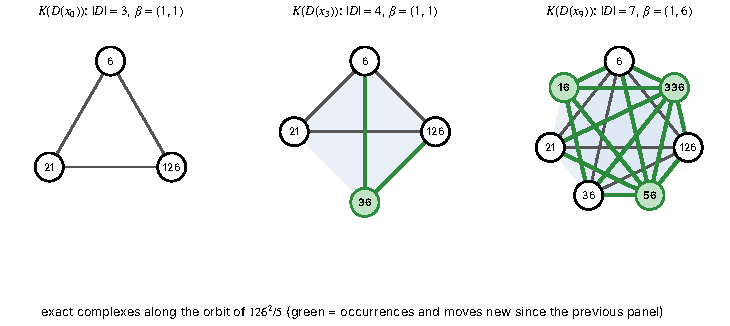
\includegraphics[width=\linewidth]{fig14_activation_orbit.pdf}
\caption{\textbf{Dormant-to-active structure along an actual collective trajectory.} Complexes $K(D(x_n))$ at $n=0,3,9$ of the orbit of $x_0=126^2/5$; green marks occurrences and moves that are new relative to the previous panel. The occurrence set grows, edges are born at arrival times. \emph{Exact complexes; vertex placement on a circle carries no meaning.}}\label{fig:orbit}\end{figure}
\begin{figure}[t]\centering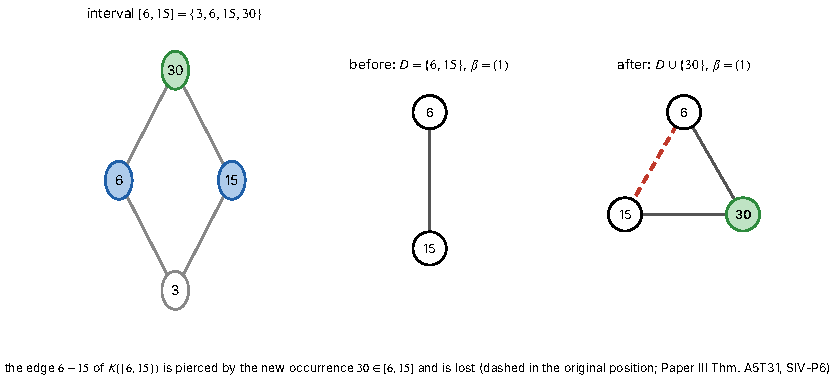
\includegraphics[width=\linewidth]{fig15_divisor_interval.pdf}
\caption{\textbf{Occurrence persistence with primitive-edge loss.} The divisor interval $I(6,15)=\{3,6,15,30\}$ and the complexes $K(\{6,15\})$ and $K(\{6,15,30\})$: the new occurrence $30$ pierces the interval and the edge $6$--$15$ is lost (dashed), replaced by $6$--$30$ and $15$--$30$ (\Src{III}{thm:A5T31}). \emph{Exact.}}\label{fig:interval}\end{figure}
\begin{figure}[t]\centering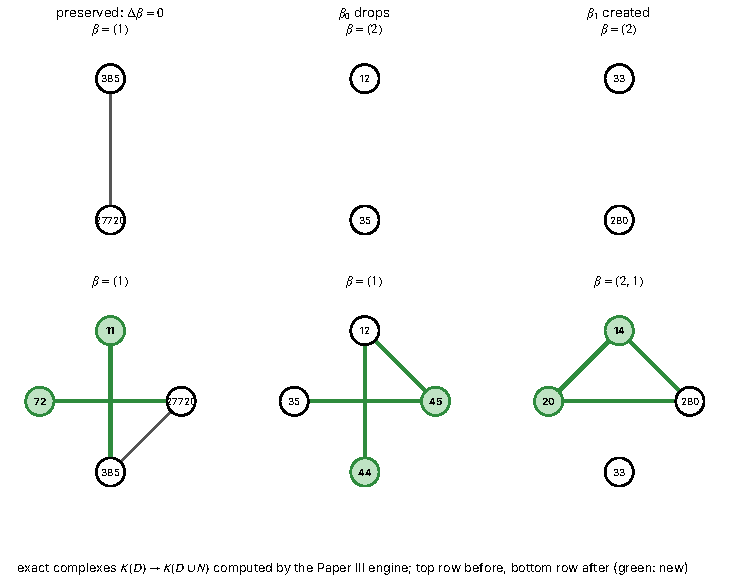
\includegraphics[width=\linewidth]{fig16_event_types.pdf}
\caption{\textbf{Topological creation, preservation and destruction.} Three exact events $K(D)\to K(D\cup N)$: unchanged Betti numbers, loss of a component, creation of a first homology class. \emph{Exact complexes computed by the engine of Paper~III; $\beta$ over $\mathbb F_2$.}}\label{fig:types}\end{figure}

\section{Arithmetic prediction and homological consequences}\label{sec:prediction}
\subsection{What arithmetic predicts}
Paper~III proves that the step at which the occurrence set next changes is given by a congruence sieve: with $Y_j=ah+jL^2$ the integers $d\ge2$ occur at the stage $j$ iff $Q(d)\mid Y_j$ (\Src{III}{thm:sieve}), so the event time is computed from divisibility alone (\Src{III}{cor:event}); and that the first occurrences that arrive in an activation family are determined by explicit moduli (\Src{III}{thm:A5T24}). The homological consequences are governed by the zig-zag identity $K\leftarrow K^\circ\to K'$ (\Src{III}{thm:zigzag}) and, for nested events, $\Delta\beta_i=h_i(K',K)-k_i-k_{i-1}$ (\Src{III}{thm:nested}). The question is how much of $\Delta\beta$ is determined by cheaper data.

\noindent\Cref{fig:event} shows arithmetic prediction of collective occurrence events.

\begin{figure}[t]\centering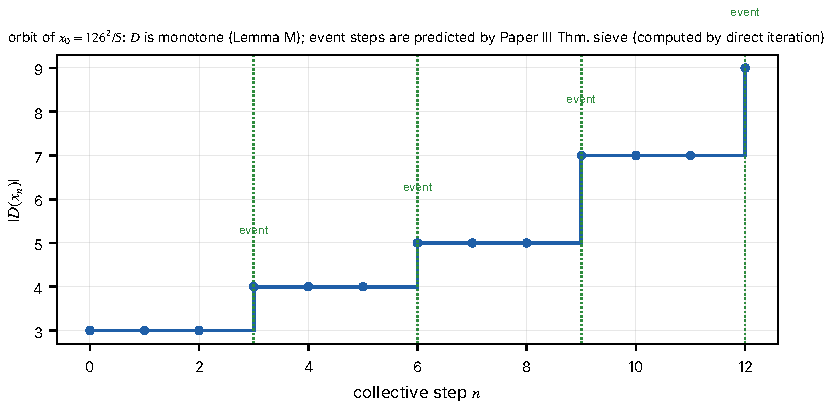
\includegraphics[width=\linewidth]{fig13_event_prediction.pdf}
\caption{\textbf{Arithmetic prediction of collective occurrence events.} The size $|D(x_n)|$ along the orbit of $126^2/5$: monotone with events at the steps predicted by the stage sieve (\Src{III}{thm:sieve}). \emph{The mechanism is the cited theorem; the plotted values are computed by direct iteration.}}\label{fig:event}\end{figure}
\subsection{Information requirements}
\begin{proposition}[\SIV{7}: information requirements for topological prediction]\label{prop:P7}\status{new, proved; witnesses finite-exact}
Let $D\subseteq D'=D\cup N$ be finite sets of integers $\ge2$ (statements (a)--(d) concern the abstract complexes $K(D),K(D')$; the witnesses of (d) are abstract and are not claimed to occur along collective orbits) with $K=K(D)$, $K'=K(D')$, local data $\lambda=(f(K),f(K'),\text{dead cells},\text{new cells})$, where $f$ is the cell-count vector.
\begin{enumerate}[label=(\alph*),itemsep=1pt]
\item \emph{Euler.} $\sum_i(-1)^i\Delta\beta_i=\sum_i(-1)^i\Delta f_i$; the right side is a function of $\lambda$.
\item \emph{First Betti number from supports.} $\Delta\beta_0=\mathrm{cl}(D')-\mathrm{cl}(D)$ where $\mathrm{cl}$ is the number of classes of the share-a-prime relation (\cref{lem:comp}); it is a function of the prime supports of $D$ and $N$ and does not need the complexes.
\item \emph{Graph level is determined.} If $K$ and $K'$ have no $2$-cells, then $\Delta\beta_1=\Delta f_1-\Delta f_0+\Delta\beta_0$ and $\Delta\beta_i=0$ for $i\ge2$. Thus $(\lambda,\text{supports})$ determine $\Delta\beta$ completely.
\item \emph{Obstruction: $\lambda$ alone does not determine $\Delta\beta$ (abstract set-level events).} The events $D=\{385,27720\}$, $N=\{11,72\}$ and $D=\{15,315\}$, $N=\{4,21\}$ have the same $\lambda$ ($f=(2,1,0)\to(4,3,0)$, nothing lost, $2$ new vertices and $2$ new edges), with $\Delta\beta=(0,0,0)$ and $(+1,+1,0)$. Likewise $D=\{12,35\},N=\{44,45\}$ and $D=\{33,280\},N=\{14,20\}$ have $f=(2,0,0)\to(4,3,0)$ and $\Delta\beta=(-1,0,0)$ versus $(0,+1,0)$.
\item \emph{Beyond graph level (open).} When $2$-cells are present, $\lambda$ together with $\Delta\beta_0$ fixes only the alternating sum $\Delta\beta_1-\Delta\beta_2+\cdots$. We know of no pair with equal $\lambda$ and equal $\Delta\beta_0$ but different $(\Delta\beta_1,\Delta\beta_2)$: a random search of $60{,}000$ events ($2{,}039$ distinct values of $(\lambda,\Delta\beta_0)$ with $2$-cells) found none. This is not a theorem (O4).
\end{enumerate}
\end{proposition}
\begin{proof}
(a) For finite complexes $\chi=\sum(-1)^i\beta_i=\sum(-1)^if_i$ over any field. (b) is \cref{lem:comp} applied to $D$ and $D'$. (c) By (a) with $f_i=0$ for $i\ge2$: $\Delta\beta_0-\Delta\beta_1=\Delta f_0-\Delta f_1$, and higher Betti numbers vanish for a graph. (d) The values of $\lambda$ and the Betti numbers of the four complexes are recomputed with the exact engine (Appendix~\ref{app:obstructions}, E5); they also illustrate (b) and (c): in the first pair $\Delta f_1-\Delta f_0=0$, so $\Delta\beta_1=\Delta\beta_0$, which is $0$ for $\mathrm{cl}:1\to1$ and $+1$ for $\mathrm{cl}:1\to2$; in the second pair $\Delta f_1-\Delta f_0=+1$ and $\mathrm{cl}:2\to1$, $2\to2$ give $\Delta\beta_1=0$ and $+1$. (e) records a search outcome.
\end{proof}
\begin{remark}
The arithmetic therefore predicts \emph{when} the occurrence set changes (sieve) and \emph{what} $\beta_0$ and, at graph level, $\beta_1$ become (supports and local counts). What is not predicted from local counts is how new cells attach to old homology classes in positive degree; that information is the attachment data $(r_i,h_i,\beta(K^\circ))$ of \Src{III}{thm:zigzag}.
\end{remark}

\noindent\Cref{fig:local} shows surviving complex and homological attachment information.

\begin{figure}[t]\centering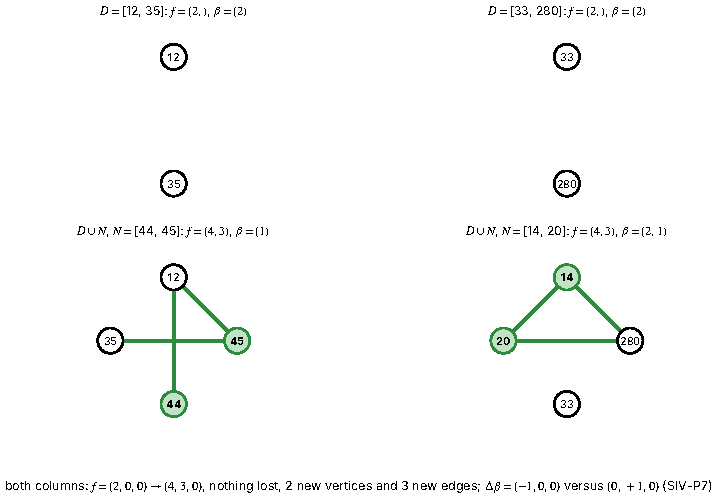
\includegraphics[width=\linewidth]{fig17_local_inventory.pdf}
\caption{\textbf{Surviving complex and homological attachment information.} Two events with identical local counts $f=(2,0,0)\to(4,3,0)$ and different Betti changes: $\Delta\beta=(-1,0,0)$ and $(0,+1,0)$. The difference is carried by the prime supports of the new vertices relative to the old components (\cref{prop:P7}(b),(c)). \emph{Exact.}}\label{fig:local}\end{figure}

\section{Collective recurrence and geometric behavior}\label{sec:recurrence}
Paper~III studies two infinite families of towers in which the orbit returns, after a fixed number of steps, to a multiple of its starting point: for $G=5$ the period is $3$ steps with multiplier $4$ (\Src{III}{thm:R3T5c}), and for $G=11$ it is $8$ steps with multiplier $9$ (\Src{III}{thm:R3T5bp}). The Betti numbers of the corresponding complexes are known exactly for $k\le140$ (\Src{III}{thm:A5T6}) and eventually quasi-polynomial without an effective threshold (\Src{III}{thm:A5T53}). The \emph{scaling data} of a tower are the period, the multiplier, the value of $G$ and the growth law of $L_k$. The question here is whether the scaling data determine the topology.

\begin{proposition}[\SIV{8}: scaling information versus geometric structure]\label{prop:P8}\status{new; proved by exact computation on stated ranges (finite-exact)}
For $S_0\in\{126,3094\}$ and $x_k=(S_02^k)^2/5$ one has $C^3(x_k)=4x_k=x_{k+1}$, $L(x_k)=S_02^k$ and $G(x_k)=5$ for $0\le k\le11$ (twelve periods); the two towers therefore have the same \emph{normalized scaling signature} $\sigma=(G,\text{period},\text{multiplier},\rho)=(5,3,4,2)$, where $\rho=L(x_{k+1})/L(x_k)$ is the growth ratio of $L$. (The towers do \emph{not} share the values of $L$ itself: $L(x_0)=126$ and $3094$ respectively.) Their complexes $K(D(x_k))$ have, for each of $k=11,\dots,14$, Betti numbers $(1,6,5,0)$ for $S_0=126$ and $(1,10,9,1,0)$ for $S_0=3094$ (over $\mathbb F_2$). Hence the parameters $G$, the period, the multiplier and the growth ratio $\rho$ do not determine the Betti vector, even for $k$ in the stable range; in particular $\beta_3$ and the total Betti sum differ. No claim is made about any other scaling parameter, in particular about the initial value $L(x_0)$ or its divisor lattice.
\end{proposition}
\begin{proof}
Direct exact computation (Appendix~\ref{app:finite}): iterating $C$ on rationals for $36$ steps from $x_0$, comparing $C^{3j+3}(x_0)$ with $4C^{3j}(x_0)$ and computing $L$, $G$; and computing $K(D)$ and its $\mathbb F_2$-Betti numbers for $S_02^k$, $0\le k\le14$. For $S_0=126$ the values $(1,6,5,0)$ at $7\le k\le140$ are proved finite-exact in \Src{III}{thm:A5T6}; our computation agrees on $7\le k\le14$. The statement concerns only the stated ranges and makes no claim about larger $k$.
\end{proof}
\begin{remark}
The seeds are $126=2\cdot3^2\cdot7$ and $3094=2\cdot7\cdot13\cdot17$. The extra prime factors of $3094$ coincide with a non-zero $\beta_3$ although the modulus $5$, the period and the multiplier are identical. We do not identify which property of the divisor lattice of $S_0$ controls the Betti vector; that is the content of the open problem O5.
\end{remark}

\noindent\Cref{fig:scaling} shows $G=5$ scaling versus geometric evolution.

\begin{figure}[t]\centering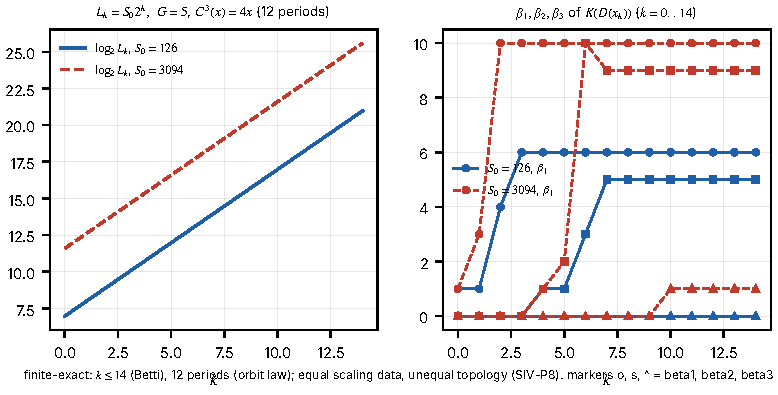
\includegraphics[width=\linewidth]{fig18_scaling_vs_topology.pdf}
\caption{\textbf{$G=5$ scaling versus geometric evolution.} Two towers with the same scaling signature $(G,\text{period},\text{multiplier},\rho)=(5,3,4,2)$ but different $L(x_0)$ (left) and different Betti numbers (right). \emph{Finite-exact: orbit law verified for twelve periods, Betti numbers for $0\le k\le14$; no extrapolation.}}\label{fig:scaling}\end{figure}

\section{Correspondence between distinct generating rules}\label{sec:correspondence}
The two rules are distinct transformations; the question is at which levels a precise relation exists. We separate five levels.
\begin{definition}[correspondence levels]
\textbf{L1} numerical ratios (values of $C^n(x)/x$ and $T_N(x)/x=R(N)$); \textbf{L2} occurrence information (the sets $D$ and their transport); \textbf{L3} reduced event records (which labels or occurrences appear when); \textbf{L4} geometric structures (complexes, Betti numbers); \textbf{L5} dynamical intertwining ($\Phi\circ C=T\circ\Phi$ for a map $\Phi$ between the state spaces).
\end{definition}
\begin{theorem}[cited: individual versus collective dynamics]\label{thm:cited-corr}
(i) For every state with $D(x)\ne\emptyset$: $1<C(x)/x\le2$, whereas $R(N)\ge4$; hence $C(x)\ne T_N(x)$ for all $N$ (\Src{III}{prop:onestep}). (ii) On the $G=5$ towers $C^3(x)=4x=T_1(x)$; $R(N)\in\Z$ iff $N=1$; the multiplier $9$ of the $G=11$ towers is not $R(N)$; and all coincidences $x_m/x_n=R(N)$ in the towers are classified in \Src{III}{thm:R3T7}.
\end{theorem}
\begin{proposition}[\SIV{9}: correspondence levels for distinct arithmetic dynamics]\label{prop:P9}\status{new for (c); assembled from cited results for (a),(b),(d)}
\begin{enumerate}[label=(\alph*),itemsep=1pt]
\item \emph{One-step identity correspondence is obstructed.} There is no $N$ with $C=T_N$ on any state with $D\ne\emptyset$; consequently the identity map $\Phi=\mathrm{id}$ (or the inclusion $\iota:\Z\to\Q_{>0}$) does not intertwine one step of $C$ with one step of any $T_N$. This excludes only the identity-type correspondence; it does \emph{not} exclude a non-identity $\Phi$ with $\Phi\circ C=T\circ\Phi$, and the existence of such a $\Phi$ (the general L5 problem) is open (O3). The snapshot relation $C^3=T_1$ on the towers is likewise not a conjugacy (\Src{III}{thm:BT12}).
\item \emph{L1 has a rigid, restricted positive result.} $C^3=T_1$ on the $G=5$ towers; for $G=11$ and the multiplier $9$ there is no ratio coincidence; the full list of coincidences is \Src{III}{thm:R3T7}.
\item \emph{L2 has a proved correspondence on integer states.} Let $x\in\Z_{\ge1}$ with $D(x)\ne\emptyset$ and $C(x)\in\Z$. Then $D(x)\subseteq D(C(x))$ and for each $d\in D(x)$ the predecessor of $C(x)$ along $d$ is the predecessor of $x$ along $d$ translated by $(d-1)L^2/(Gd^2)$: with $\mathrm{pred}_d(t)=t(d-1)/d^2$,
\[\mathrm{pred}_d(C(x))=\mathrm{pred}_d(x)+\frac{(d-1)L^2}{G\,d^2}.\]
Hence the incoming steps of $x$ inject into those of $C(x)$ ($d\mapsto d$) and the collective map acts on the ancestry fan of an integer as a monotone enlargement with explicit translation.
\item \emph{L3 and L4: restricted positive results, no general map.} On the rigid domain $x=t\sigma^2$, $t\in\{1,2,3\}$, $\sigma$ even, the collective segment $x\to C^3(x)=4x$ and the edge $T_1:x\mapsto4x$ have the same reduced event record, and at integer endpoints the complexes agree (\Src{III}{thm:B2T10}); for the tower pairs with a SELECT-II ratio the event counts agree in the cases listed in \Src{III}{thm:R3T7}, and fail for $N=8$ ($G=11$) and $N=3$ ($G=5$) although the ratios agree. Beyond these cases no map between event records, and none between the history complexes of $t$ and the evolving complexes $K(D(x_n))$, is established; the endpoint geometry cannot be a history invariant (\cref{prop:P5}), and general constructions are open (O3).
\end{enumerate}
\end{proposition}
\begin{proof}
(a) and (b) are \cref{thm:cited-corr}. (c) By \cref{lem:M-cited} $D(x)\subseteq D(C(x))$; by \cref{prop:P2}(a) the incoming steps of an integer $t$ are indexed by $D(t)$ with predecessor $t(d-1)/d^2$. Therefore each $d\in D(x)$ indexes an incoming step of $C(x)$, and $\mathrm{pred}_d(C(x))=(x+L^2/G)(d-1)/d^2$, which is $\mathrm{pred}_d(x)+(d-1)L^2/(Gd^2)$. For $d\in D(x)$ the quantity $\mathrm{pred}_d(C(x))$ is an integer because $d^2\mid C(x)$. (d) The positive statements are \Src{III}{thm:B2T10} and \Src{III}{thm:R3T7}, quoted; the negative statement is \cref{prop:P5}, and the remaining open questions are in Section~\ref{sec:open}. (a) is an obstruction to one specific family of maps only: it uses the ratio bound, which a non-identity $\Phi$ is not required to respect.
\end{proof}
\begin{remark}
\cref{prop:P9}(c) is genuinely about the overlap of the two domains, the integers; it uses the generative interpretation of $D(t)$ and the collective step in one formula, but it does not say that $C(x)$ is a generative successor of $x$, which (a) excludes. We recomputed (c) on $1008$ integer states with integer image (Appendix~\ref{app:finite}).
\end{remark}

\noindent\Cref{fig:levels} shows the five levels of cross-system correspondence.

\begin{figure}[t]\centering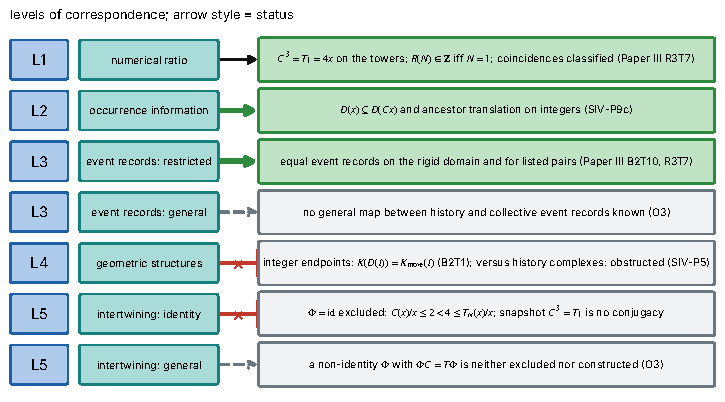
\includegraphics[width=\linewidth]{fig19_correspondence_levels.pdf}
\caption{\textbf{The five levels of cross-system correspondence.} Arrow style gives the status of what is known: established (L1), proved restricted statements (L2; L3 on the rigid domain and listed pairs), open (L3 in general; L5 for a non-identity $\Phi$), obstructed (L4 against history complexes; L5 for $\Phi=\mathrm{id}$). \emph{Schematic of status; each row cites the proposition or theorem that supports it.}}\label{fig:levels}\end{figure}

\section{The unified diagram}\label{sec:diagram}
\subsection{Objects, maps and statuses}
The diagram of \cref{fig:global} has two columns of objects. On the generative side: histories, swap classes, contents, endpoints, occurrence sets of integers, endpoint complexes and their Betti numbers, and the route complexes and counts of the history space of a fixed source and endpoint. On the collective side: rational states, their occurrence sets, their move complexes and primitive systems, and the same data at the image under $C$. Integers belong to both sides.

Every arrow carries one of five statuses (see \cref{sec:intro} for the line conventions): \emph{established arrow} (a source-defined function, cited or defined here); \emph{proved factorization} (a map that factors through another under stated hypotheses); \emph{proved obstruction} (a reconstruction ruled out by an exact result); \emph{open construction}; \emph{interpretive comparison} (no formal correspondence claimed).
\subsection{Factorizations}
\cref{fig:fact} shows the factorization chain of \cref{sec:numerical,sec:occurrence} with the sets on which it is defined: the maps $\mathrm{Hist}(m_0)\to\mathrm{Cls}\to\mathrm{Cont}\to\Z\to\{D\}$ are for a fixed source $m_0$ (or all integers in the last step), and $D\mapsto K(D)\mapsto\beta$ are functions of $D$ (\Src{III}{thm:R3T1a}). The two obstructions leaving this chain are the primitive system (\cref{prop:P2}(c)) and the history counts (\cref{prop:P5}).
\begin{figure}[t]\centering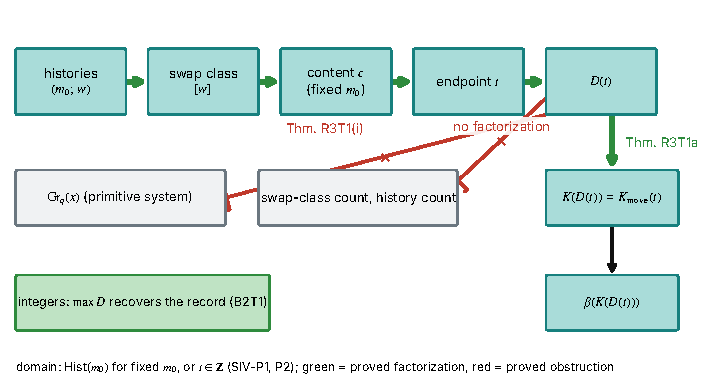
\includegraphics[width=\linewidth]{fig20_factorization_D.pdf}
\caption{\textbf{A source-supported factorization diagram.} What passes through the occurrence set $D$ and what does not. Green: proved factorizations; red: proved obstructions (\Src{III}{thm:R3T1}(i) and \cref{prop:P5}). \emph{Exact content: statuses and domains; boxes are schematic.}}\label{fig:fact}\end{figure}
\subsection{Commuting relations}
\begin{proposition}[no claimed commuting squares]\label{prop:nocomm}
Let $\iota:\Z\to\Q_{>0}$ be the inclusion. The following squares are \emph{not} claimed to commute and the corresponding statements are false or unestablished: (i) $C\circ\iota=\iota\circ T_N$ for any $N$ (false by \cref{prop:P9}(a); this excludes the identity-type correspondence only, not a non-identity $\Phi$); (ii) $K(D(\cdot))\circ\mathrm{end}$ determines the history complex (false by \cref{prop:P5}); (iii) $D\mapsto\Gr$ (does not exist, \cref{prop:P2}(c)). The only commuting relations proved in this manuscript are the factorization identities $\Endp=\pi_3\pi_2\pi_1$ and $\mathrm{(realised\ record)}=g\circ D$.
\end{proposition}
\begin{proof}
(i) is \cref{thm:cited-corr}(i). (ii) is \cref{prop:P5}. (iii) is \cref{prop:P2}(c). The two commuting identities are \cref{prop:P1}(a) and \Src{III}{thm:R3T1a}.
\end{proof}
\begin{figure}[p]\centering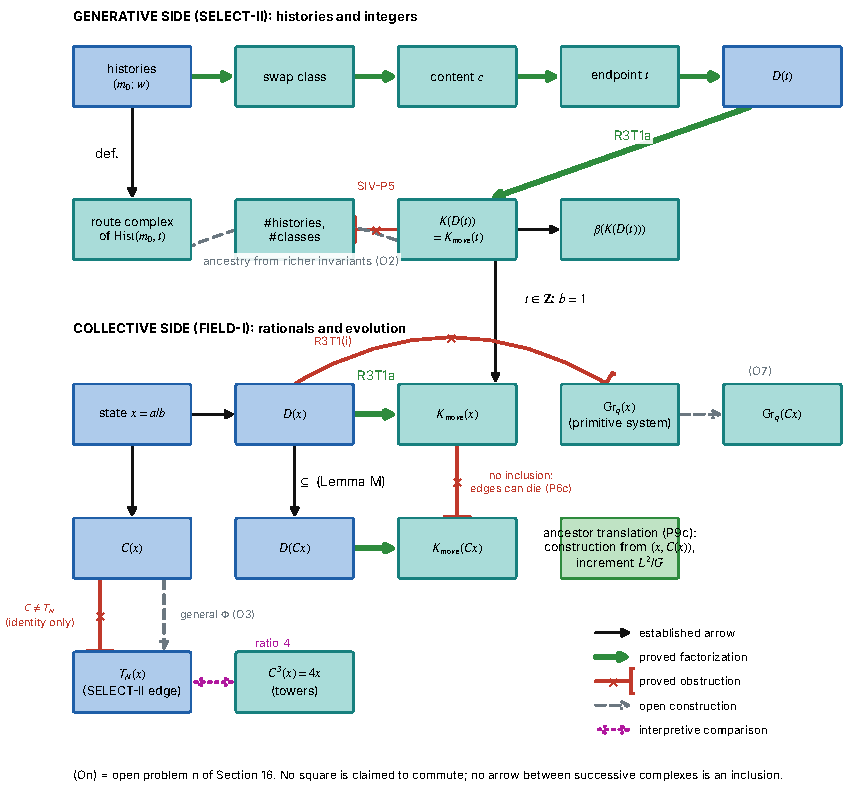
\includegraphics[width=\linewidth]{fig21_global_diagram.pdf}
\caption{\textbf{The global diagram of maps, factorizations and obstructions.} Objects are the structures of \cref{sec:objects}; each arrow is labelled with its status by line style and cited result. Green arrows: factorizations proved from the cited theorems; black arrows: established functions; red arrows with a cross: proved obstructions (R3T1(i) is \Src{III}{thm:R3T1}(i); SIV-P5 is \cref{prop:P5}; $C\ne T_N$ is \cref{prop:P9}(a)); grey dashed arrows: open constructions (O2, O3, O7); purple dotted arrow: interpretive comparison of the ratio $4$ (\cref{thm:cited-corr}(ii)). The arrow between $K_{\rm move}(x)$ and $K_{\rm move}(Cx)$ is drawn as an obstruction to an \emph{inclusion}: vertices persist but edges can be lost (\cref{prop:P6}(c)), so no complex inclusion is implied. The box \emph{ancestor translation} is a construction from the arithmetic pair $(x,C(x))$ and the set $D(x)$ (\cref{prop:P9}(c)), not a function of $K_{\rm move}(Cx)$, and is therefore drawn without an arrow from that complex. The legend is in the figure. \emph{Schematic of status: the diagram is a map of established relations, not a commuting diagram; the status of each arrow is defined in Appendix~\ref{app:diagram}.}}\label{fig:global}\end{figure}

\section{Synthesis propositions and obstructions}\label{sec:register}
\cref{tab:register} lists the nine synthesis propositions with their status and what each rests on; the machine-readable register is \texttt{crosswalk/SYNTHESIS\_PROPOSITIONS.tsv}. A proposition is marked \emph{new} when its statement is derived here with an independent proof; no result is silently upgraded from a finite-exact status.
\begin{table}[t]\centering\footnotesize\setlength{\tabcolsep}{3pt}\begin{tabular}{@{}p{1.3cm}p{4.6cm}p{4.6cm}p{2.5cm}@{}}\toprule
ID & Subject & Status & Statement \\\midrule
SIV-P1 & Endpoint projection and retained information & NEW-PROVED & \cref{prop:P1}\\
SIV-P2 & Occurrence projection and primitive-relation information & NEW-PROVED (a); CITED (b),(c) & \cref{prop:P2}\\
SIV-P3 & Arithmetic availability versus geometric realization & NEW-PROVED (a),(b); CITED (c),(d) & \cref{prop:P3}\\
SIV-P4 & Arithmetic constraints and global history connectivity & NEW-PROVED from cited theorems; FINITE check & \cref{prop:P4}\\
SIV-P5 & Limits of endpoint geometry as a history invariant & NEW-PROVED (exhaustive recursion); FINITE-EXACT census & \cref{prop:P5}\\
SIV-P6 & Hierarchy of structural persistence under evolution & NEW-PROVED; (d) quotes finite-exact census & \cref{prop:P6}\\
SIV-P7 & Information requirements for topological prediction & NEW-PROVED (a)-(d); (e) search outcome only & \cref{prop:P7}\\
SIV-P8 & Scaling information versus geometric structure & NEW; FINITE-EXACT (k<=14, 12 periods) & \cref{prop:P8}\\
SIV-P9 & Correspondence levels for distinct arithmetic dynamics & NEW-PROVED (c); ASSEMBLED (a),(b),(d) & \cref{prop:P9}\\
\bottomrule\end{tabular}\caption{\textbf{Register of the synthesis propositions.} New results are proved in the text or in Appendix~\ref{app:proofs}; inherited ingredients are cited by theorem number (Appendix~\ref{app:prov}); finite-exact statements are labelled with their checked ranges.}\label{tab:register}\end{table}

\subsection{Answers to S1--S4}
\begin{description}[leftmargin=1.2em,itemsep=2pt]
\item[S1] \emph{Proved for integer states, open beyond.} The generative guard $(N+1)^2\mid t$ and the occurrence guard $d^2\mid t$ coincide under $d=N+1$ (\cref{prop:P2}(a)). For rational states the guard $d\equiv1\pmod b$ has no generative counterpart; a rational extension of the generative rule reproducing it is open (O8).
\item[S2] \emph{Proved, with obstructions.} The endpoint retains the valuation displacement $V_Ac$ and nothing finer (\cref{prop:P1}); the occurrence set retains everything that enters $\Kmove$ and nothing about the primitive system or about the number of histories (\cref{prop:P2,prop:P5}). Reconstruction of a history needs the fibre sequence along the path (\cref{thm:faith-cited}).
\item[S3] \emph{Proved obstruction and open maps.} $K(D(t))$ does not determine the topology of $\Hist(m_0,t)$ (\cref{prop:P5}); the route-complex side has independent arithmetic (\cref{prop:P4}); explicit maps between history geometry and evolving occurrence geometry beyond L2 are open (\cref{prop:P9}, O3).
\item[S4] \emph{Conditional (structural).} Both criteria are instances of monotone minimality (\cref{cor:S4}); an exact implication between them requires an identification of ambient orders and is open (O7).
\end{description}

\section{Relation to established theories}\label{sec:theories}
Each comparison is classified as \textbf{identical} (an established equivalence), \textbf{special case} (a proved inclusion), \textbf{analogy} (similar behaviour without a proved equivalence) or \textbf{open}. Nothing in the manuscript is proved by appeal to these theories, and no claim of priority is made.
\begin{description}[leftmargin=1.2em,itemsep=3pt]
\item[Arithmetic dynamics and divisibility systems.] The map $C$ is a rational map of the positive rationals defined by arithmetic data; its occurrence set is a divisor condition on the numerator. \emph{Analogy}: we do not connect $C$ with the standard theory of dynamics of rational functions; the comparison with $p$-adic or arithmetic-dynamical invariants is \emph{open}.
\item[Geometry of numbers and lattice relations.] The lattice $\Lambda_b\subseteq\Z^k$ of exponent vectors with product $\equiv1\bmod b$ is the kernel of a homomorphism to $(\Z/b)^\times$; its transport (\Src{I}{thm:P2T1}) is a statement about kernels of homomorphisms. \emph{Identical} with the standard description of such sublattices (cf.\ Cassels, \emph{An Introduction to the Geometry of Numbers}); the dimensional results are UNNS-specific.
\item[Graver bases.] The set $\Gr_q$ is the Graver basis of the lattice restricted to a box \cite{Graver1975,Sturmfels1996}, and the persistence criterion \Src{I}{thm:P2T2} is a statement about conformal minimality. \emph{Special case} of the notion of a Graver basis; the monotone-minimality principle (\cref{lem:minimal}) is a general, elementary statement which these criteria instantiate.
\item[Rewriting systems and confluence; trace monoids.] Swap classes are the classes of a rewriting system generated by commutation of adjacent letters when both orders are admissible, as in partially commutative (trace) monoids \cite{DiekertRozenberg1995}. The commutation here is \emph{state-dependent}, so a history space is not a free partially commutative monoid; \emph{analogy}. Confluence of the block rewrites is studied in Paper~II; whether the swap graph can be described by a trace-type normal form is \emph{open}.
\item[Cubical and cellular complexes; homology.] The complexes $K(D)$ are cubical in the sense of Paper~III's definition; homology is computed over $\mathbb F_2$ (and checked over another field in the sources), and cellular homology and the long exact sequence of a pair are standard \cite{Hatcher2002}. \emph{Identical} use of standard tools; the divisor-interval cell structure is specific.
\item[Zig-zag and filtered structures.] The shape $K\leftarrow K^\circ\to K'$ of an event resembles a zig-zag diagram of complexes \cite{CarlssonDeSilva2010}; we use only that shape. \emph{Analogy}; no use is made of zig-zag persistence theory.
\item[Information-losing projections.] The factorization lemma \cref{lem:factor} is the universal property of a quotient by the fibre relation of a surjection; \emph{identical}.
\end{description}

\section{Principal mathematical conclusions}\label{sec:conclusions}
Each conclusion cites the result on which it rests; broad readings are labelled as interpretation.
\subsection{Operational characterisation of the UNNS Substrate}\label{sec:characterisation}
The preceding results support an operational characterisation of the UNNS Substrate as a rule-governed generative arithmetic architecture. Its mathematical organisation is not exhausted by numerical states, individual generating histories, occurrence inventories, primitive arithmetic relations, or realised geometric complexes considered separately. It is expressed through the admissible transformations and structural relationships among these objects.

The generative framework may be represented schematically by
\[
\mathcal U=(S,\mathcal O,\mathrm{Dom},\mathcal R,\mathsf{Adm}),
\]
where $S$ is a set of states, $\mathcal O$ a set of operators, $\mathrm{Dom}$ the assignment of a domain to each operator, $\mathcal R$ the set of admissible routes, and $\mathsf{Adm}$ the conditions governing admissibility. In the arithmetic constructions studied here, $S$ consists of the positive integers and rationals, $\mathcal O$ of the maps $T_N$ and $C$, $\mathrm{Dom}$ of the conditions $N\mid m$ and $D(x)\neq\emptyset$, $\mathcal R$ of histories and collective orbits, and $\mathsf{Adm}$ of the divisibility conditions on squares. The tuple is a notation for organising what has been proved; it is not an axiom system from which the results are derived. The occurrence and geometric structures studied here ($D$, the lattice of relations, the primitive system $\mathrm{Gr}_q$, the complexes $K(D)$ and their Betti numbers) are associated constructions, not additional primitive components assumed without definition.

The results establish the following characteristic properties of this architecture; each is a restatement of the cited result for the stated domain.
\begin{center}\footnotesize\setlength{\tabcolsep}{4pt}\begin{tabular}{@{}p{7.2cm}p{4.6cm}@{}}\toprule
Property & Support\\\midrule
Numerical endpoints need not identify their generative histories; the endpoint retains only the valuation displacement. & \cref{prop:P1}, \cref{prop:P5}\\
Occurrence inventories determine the realised move complexes, but not the complete primitive relation systems. & \cref{prop:P2}(b),(c); \Src{III}{thm:R3T1a}, \Src{III}{thm:R3T1}\\
Arithmetic relations can remain dormant until further occurrences permit their geometric realisation. & \cref{prop:P3}; \Src{I}{thm:P2T2}\\
Global connectivity of the history space is governed by arithmetic of the source, not by local swaps alone. & \cref{prop:P4}\\
Under the collective map, occurrence sets grow, connectivity only coarsens, and each edge exists during an arithmetically determined interval. & \cref{prop:P3}(b), \cref{prop:P6}(a)--(c)\\
Event steps follow exact arithmetic laws, and at graph level the change of the first two Betti numbers follows from local counts and prime supports; local counts alone do not determine it, and beyond graph level the determination is open. & \cref{prop:P7}; \Src{III}{thm:sieve}\\
Scaling parameters do not determine topology (finite-exact). & \cref{prop:P8}\\
The two rules are related at integers and occurrence labels, not by a one-step identity correspondence. & \cref{prop:P9}; \cref{fig:global}\\
\bottomrule\end{tabular}\end{center}

These properties show that generation, arithmetic possibility, geometric realisation and structural evolution are distinct but mathematically related aspects of the framework. Their relationships are governed by the proved factorizations, admissibility conditions, transition laws and obstructions of \cref{sec:numerical,sec:occurrence,sec:realization,sec:history,sec:endpoint,sec:evolution,sec:prediction,sec:recurrence,sec:correspondence}, collected in \cref{fig:global}.

Consequently, the UNNS Substrate is characterised operationally not by a single geometric object, but by a system of admissible generative mechanisms and the layered structures they produce and transform.

\emph{Scope.} This characterisation is supported by the results established for the specified arithmetic constructions. It does not assert that every component derives from a unique minimal axiom system, that all generative operators are dynamically equivalent, or that the mathematical framework has been identified with a physical substrate. Establishing a fully intrinsic characterisation remains a separate mathematical problem (\cref{sec:intrinsic}).

\subsection{Mathematical implications}\label{sec:implications}
Each conclusion cites the result on which it rests; broad readings are labelled as interpretation.
\begin{enumerate}[label=\textbf{C\arabic*.},itemsep=3pt]
\item \textbf{Generation.} Arithmetic conditions decide which steps and which histories exist: a step $m\xrightarrow{N}t$ exists iff $d=N+1$ satisfies $d^2\mid t$ (\cref{prop:P2}(a)), and legal swaps are decided by divisibility at each state (\cref{prop:P4}).
\item \textbf{Ancestry.} The numerical endpoint determines only the valuation displacement of the history (\cref{prop:P1}); equal occurrence sets are compatible with different numbers of histories and of swap classes (\cref{prop:P5}).
\item \textbf{Geometry.} The realised geometry of a state is a function of its occurrence set (\Src{III}{thm:R3T1a}); the primitive relation system contains information that the occurrence set does not (\cref{prop:P2}(c)).
\item \textbf{Transport.} Preservation under lattice inclusion holds in rank two (\Src{I}{thm:planar}) and fails in rank three under the hypotheses of \Src{I}{thm:C1}; abstract and realised loss differ (\Src{I}{prop:topology}).
\item \textbf{Recombination.} Local legal swaps do not force a connected history space: the class count of $\{2,3,14\}$ is $0$, $1$ or $2$ according to arithmetic of the source and is not monotone in divisibility (\cref{prop:P4}).
\item \textbf{Evolution.} Collective steps enlarge the occurrence set, only coarsen the connectivity relation, give each edge an interval of existence, and leave higher Betti numbers unconstrained by monotonicity (\cref{prop:P3,prop:P6}).
\item \textbf{Prediction.} Arithmetic congruences give the event step; supports and local counts give $\Delta\beta_0$ and, at graph level, $\Delta\beta_1$; positive-degree homology needs attachment data (\cref{prop:P7}, \Src{III}{thm:sieve}, \Src{III}{thm:zigzag}). Scaling data do not determine topology (\cref{prop:P8}).
\item \textbf{Compatibility.} The one-step identity correspondence of the two rules is obstructed (a non-identity intertwining is open); the overlap on integers admits a translation formula; the other levels are obstructed or open (\cref{prop:P9}).
\end{enumerate}
\paragraph{Answer to the governing question.} \emph{Interpretation, supported by C1--C8 and not a theorem:} in the part of the theory that is established, geometry is formed from arithmetic by two successive forgetful maps---from histories to endpoints, from states to occurrence sets---and the formation of geometry is stable in a precise sense (occurrence sets only grow; connectivity only coarsens) but not rigid (edges and higher homology are created and destroyed). Where the two generating rules meet, they meet in integers and in occurrence labels, and the exact obstructions show that nothing richer follows from the labels alone.

\subsection{Limitations}\label{sec:limitations}
The conclusions concern the specified arithmetic constructions and the finite-exact ranges stated in the propositions. Verification inherited from Papers~I--III is not re-run here (NOT\_RERUN). The collective rule is studied on its recorded domains and the generative rule on integer sources; the extension of the generative rule to rational sources is open (O8). No claim is made that the operators $T_N$ and $C$ belong to one dynamical system, that the associated constructions are independent of one another beyond the stated obstructions, or that the characterisation applies outside the constructions named. Constant C3 is unclaimed.

\section{Open questions}\label{sec:open}
Each problem states the nearest proved theorem and the missing obligation. Problems already settled by the cited releases are not repeated.
\begin{description}[leftmargin=1.2em,itemsep=3pt]
\item[O1. Classification of history complexes.] \emph{Nearest:} the fixed-content classification of $\{2,3,14\}$ (\Src{II}{thm:2314}) and the scoped block rewrites (\Src{II}{thm:block}). \emph{Missing:} a classification of swap classes and route homology for arbitrary content and source.
\item[O2. Reconstruction of ancestry from richer invariants.] \emph{Nearest:} faithfulness of the fibre sequence (\cref{thm:faith-cited}) and the obstruction \cref{prop:P5}. \emph{Missing:} a characterisation of the invariants of an endpoint, strictly between $D(t)$ and the whole fibre sequence, that determine the number of histories or of classes.
\item[O3. Maps between the two geometries.] \emph{Question:} maps between history geometry and evolving occurrence geometry, and non-identity intertwining of the two dynamics. \emph{Nearest:} the translation formula \cref{prop:P9}(c) and the restricted event correspondences \Src{III}{thm:B2T10}, \Src{III}{thm:R3T7}. \emph{Missing:} a map at level L3 or L4 beyond the rigid domain and the listed pairs, and either a construction or a non-existence proof for a non-identity $\Phi$ with $\Phi\circ C=T\circ\Phi$ (the obstruction \cref{prop:P9}(a) excludes only $\Phi=\mathrm{id}$).
\item[O4. Prediction of higher-dimensional Betti changes.] \emph{Nearest:} \cref{prop:P7}(c) and the zig-zag identity. \emph{Missing:} determination of $\Delta\beta_i$, $i\ge1$, when $2$-cells are present, from data cheaper than the full target.
\item[O5. Effective onset and closed Betti laws for towers.] \emph{Nearest:} \Src{III}{thm:A5T53} (qualitative quasi-polynomials) and \Src{III}{thm:A5T6} (exact to $k\le140$), \cref{prop:P8}. \emph{Missing:} an effective threshold, exact formulas for all $k$, and an invariant of $S_0$ that governs the Betti vector.
\item[O6. Reachability of activation families.] \emph{Nearest:} \Src{III}{thm:A4T1} and \Src{III}{thm:A5T24}. \emph{Missing:} a complete arithmetic classification of the families that occur along actual orbits.
\item[O7. Transition laws for dormant primitive systems.] \emph{Nearest:} \Src{I}{thm:P2T2}, \cref{lem:minimal}, \cref{cor:S4}. \emph{Missing:} an identification of the order on lattice vectors with the divisor-interval order on pairs of occurrences under compatible hypotheses, or an obstruction to one.
\item[O8. Compatibility of arithmetic guards.] \emph{Nearest:} the bijection \cref{prop:P2}(a) at the level of integers. \emph{Missing:} an extension of the generative rule to rational sources whose predecessor guard reproduces $d\equiv1\pmod b$.
\end{description}

\noindent\Cref{fig:frontier} shows established conclusions and open construction obligations.

\begin{figure}[t]\centering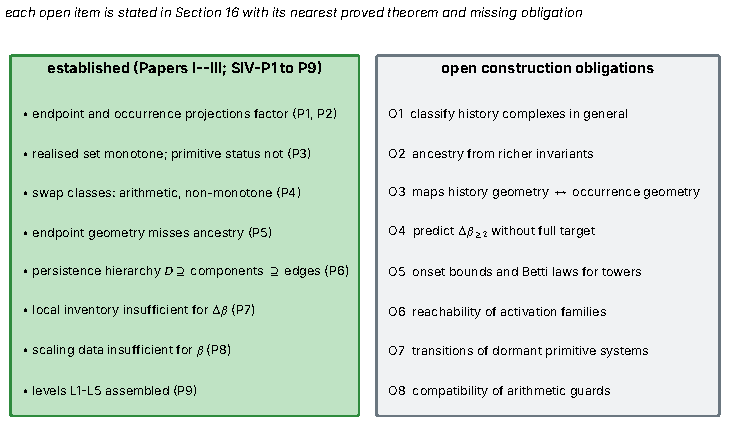
\includegraphics[width=\linewidth]{fig22_conclusions_open.pdf}
\caption{\textbf{Established conclusions and open construction obligations.} Left: the nine propositions; right: the eight open problems of this section. \emph{Schematic summary; each item is defined and referenced in the text.}}\label{fig:frontier}\end{figure}

\subsection{Operational versus intrinsic characterisation}\label{sec:intrinsic}
\Cref{sec:characterisation} characterises the Substrate \emph{operationally}: through the operators, domains, routes and admissibility conditions that are actually used, and the proved relations among the structures they generate. An \emph{intrinsic} characterisation would instead derive these components, and the associated constructions, from a minimal list of axioms and show which of them are independent. The two are different mathematical problems, and only the first is addressed here. \emph{Nearest proved results:} the factorizations and obstructions of \cref{prop:P1,prop:P2,prop:P5} and the status map of \cref{fig:global}. \emph{Missing obligations:}
\begin{enumerate}[label=(\roman*),itemsep=1pt]
\item an axiomatic definition of admissibility from which the guards $N\mid m$ and $d^2\mid a$, $d\equiv1\ (b)$ both follow (the identification is proved only for integer states, \cref{prop:P2}(a); see O8);
\item a compatibility statement placing $T_N$ and $C$ in one admissibility system, or a proof that no non-identity intertwining exists (O3);
\item a proof that the associated constructions (occurrence set, relation lattice, primitive system, complex) are determined by, or independent of, the schematic components $(S,\mathcal O,\mathrm{Dom},\mathcal R,\mathsf{Adm})$, rather than assumed through definitions;
\item the passage from the finite-exact ranges recorded here to statements for all sources, which no result of this paper provides.
\end{enumerate}

\clearpage
\phantomsection\addcontentsline{toc}{section}{References}
\begin{thebibliography}{99}\small\raggedright
\bibitem{PaperI} UNNS Research Collective, \emph{Arithmetic Transport and Dimensional Obstructions in UNNS Occurrence Geometry}, Manuscript~I of the programme GEO-HD-1, version~0.4 (2~Nov.\ 2026); file \texttt{PAPER\_I\_TRANSPORT\_v0.4.pdf}, SHA-256 \texttt{19fc10f546696909eef39c75ebdb47b5468d93173f9bd9e82567bd5f60f9eef9}.
\bibitem{PaperII} UNNS Research Collective, \emph{Generative Histories, Arithmetic Recombination, and Higher-Dimensional Route Topology}, Manuscript~II of the programme GEO-HD-1, version~0.4 (2~Nov.\ 2026); file \texttt{PAPER\_II\_HISTORIES\_v0.4.pdf}, SHA-256 \texttt{df34fa94fed9fb33b82c87726ca9e725307723f4e3cb67e1af2f55d7b56801e4}.
\bibitem{PaperIII} UNNS Research Collective, \emph{Geometric Evolution under Collective UNNS Dynamics: Activation, Events, and Topological Prediction}, Manuscript~III of the programme GEO-HD-1, version~0.4 (3~Nov.\ 2026); file \texttt{PAPER\_III\_EVOLUTION\_v0.4.pdf}, SHA-256 \texttt{47fae77fd9c11f0cc7e81447fd697cdbae413e2646564b1d966836ebad14cb8e}.
\bibitem{FoundI} UNNS Substrate programme, \emph{Mathematical Foundations of the UNNS Substrate, Volume~I: Generative Arithmetic and Structural Reachability} (the grammar SELECT-II and the occurrence set). Source: \texttt{ukbbi/UNNS}, commit \texttt{9a021346b2b3d964523440d2737b9d0c4ddbb3e5}, \texttt{projects/UNNS\_MATH\_FOUNDATIONS/Manuscript}.
\bibitem{FoundII} UNNS Substrate programme, \emph{Mathematical Foundations of the UNNS Substrate, Volume~II: Collective Dynamics, Prime Rigidity, and Effective Predictability} (the collective map FIELD-I). Same commit and path as~\cite{FoundI}.
\bibitem{GEOI} GEO-I, Papers~A and~B of the geometry programme (occurrence geometry, region-Graver sets and the realised complexes), cited at commit \texttt{9a021346b2b3d964523440d2737b9d0c4ddbb3e5} as in~\cite{FoundI}.
\bibitem{RefColl} Foundations reference collection v001 (SELECT-I/II, FIELD-I v001--v012; frozen), \texttt{ukbbi/UNNS}, commit \texttt{bb8b12d753c600c597feb00df17fe139c7cc65fa} (23 Oct.\ 2026), \texttt{projects/UNNS\_MATH\_FOUNDATIONS/sources}.
\bibitem{HD1} GEO-HD-1 research collection, snapshot \texttt{a88f31487f3b05c9db297dcd1192d56eea2b0c7d} (the pin named in the programme specification; not independently verified in this work). Frozen releases from which the inherited records are taken, with SHA-256 as computed on the files supplied for Paper~III:
\begin{itemize}[leftmargin=1.4em,itemsep=1pt,topsep=2pt]\footnotesize
\item\texttt{GEO\_HD\_1D\_v001} \texttt{c532b7410f3bf9d437f9f172b3e56029cd9f7bab5b2ac0c0e533713155eaf7a4}; \texttt{GEO\_HD\_1D\_v002} \texttt{8baf463c07bb5285dd53b355aee05a0f841c068ba3ae4794f3702adff6a4bae0}; \texttt{GEO\_HD\_1D\_v003} \texttt{65dbb281e4c75d625b6cf3e4bcb8262d7d42e68d0c476fbba225fcde744a4706}; \texttt{GEO\_HD\_1D\_v004} \texttt{e0390e2a2f88eaeb11042de09fd056741ed98f94318de708d308faa090f05b5b};
\item\texttt{GEO\_HD\_BRIDGE\_v001} \texttt{e99472809928f4a23fb292f60759965159c7a4db5f018d56748ccac328719395}; \texttt{v002} \texttt{012ead97e5b8854cd5218417d46f0e388d927b6d59d5f6e75a8cc343f5dd4955} (with errata for B2-T9 and B2-T7); \texttt{v003} \texttt{6fba87af9f3096772e43f4ac77fa8d55aea9e242eeef241081a987b567d5d5a8}; \texttt{v004} \texttt{cfb31157a39666d1a4bbb33b280ec626c7de2c141e8232da43c8b934b8affff4}; \texttt{v005} \texttt{50e342821d7a5f760c5127df348e97f3a4d4d3bf34bf60e1019d6336f28c5d03}.
\end{itemize}
\bibitem{Graver1975} J.~E. Graver, On the foundations of linear and integer linear programming~I, \emph{Math.\ Programming} \textbf{9} (1975), 207--226.
\bibitem{Sturmfels1996} B.~Sturmfels, \emph{Gr\"obner Bases and Convex Polytopes}, University Lecture Series~8, American Mathematical Society, 1996 (Graver bases, \S4).
\bibitem{Cassels1959} J.~W.~S. Cassels, \emph{An Introduction to the Geometry of Numbers}, Grundlehren der mathematischen Wissenschaften~99, Springer, 1959 (lattices; sublattices as kernels).
\bibitem{DiekertRozenberg1995} V.~Diekert, G.~Rozenberg (eds.), \emph{The Book of Traces}, World Scientific, 1995 (partially commutative monoids).
\bibitem{Hatcher2002} A.~Hatcher, \emph{Algebraic Topology}, Cambridge University Press, 2002 (cellular homology, \S2.2; long exact sequence of a pair, \S2.1).
\bibitem{CarlssonDeSilva2010} G.~Carlsson, V.~de~Silva, Zigzag persistence, \emph{Found.\ Comput.\ Math.} \textbf{10} (2010), 367--405 (zig-zag diagrams of complexes; cited for the shape $K\leftarrow K^\circ\to K'$ only).
\end{thebibliography}
\paragraph{On the references.} Papers~I--III are cited at version~0.4 by theorem number; every such number is generated from the corresponding \texttt{.aux} file (\texttt{scripts/gen\_xref.py}), so a citation that does not resolve is reported at build time. UNNS foundation sources are cited at the commits and archive hashes fixed by the programme; repository access during this work was read-only and the pinned repositories were not fetched. External literature is cited only for the standard notions named and for resemblance of structures; no statement is proved by appeal to an equivalence with those theories.

\appendix
\section{Notation}\label{app:notation}
\begin{center}\small\begin{tabular}{@{}lp{10.2cm}@{}}\toprule
Symbol & Meaning (source)\\\midrule
$T_N(m)$, $R(N)$ & $m(N+1)^2/N$ ($N\mid m$); $R(N)=(N+1)^2/N$ (Foundations~I)\\
$\Hist(m_0)$, $\Hist(m_0,t)$ & histories from $m_0$; those ending at $t$ (Paper~II)\\
$c(h)$, $F(h)$, $\Endp(h)$ & content, fibre sequence, endpoint of a history\\
$V_A$, $\Delta_p(N)$ & displacement matrix, $\Delta_p(N)=2v_p(N+1)-v_p(N)$ (Paper~II)\\
$\nu(m)$ & number of swap classes of $\{2,3,14\}$ at source $m$\\
$D(x)$ & $\{d\ge2:d^2\mid a,\ d\equiv1\ (b)\}$ for $x=a/b$ (Foundations~II)\\
$L,G$, $C(x)$ & $\lcm D$, $\gcd\{d-1\}$, $x+L^2/G$\\
$I(u,v)$ & $\{z:\gcd(u,v)\mid z\mid\lcm(u,v)\}$ (divisor interval)\\
$K(D)$, $\Kmove(x)$ & divisor-interval complex; $\Kmove(x)=K(D(x))$ (Paper~III)\\
$\Lambda_b$, $\Gr_q(x)$ & relation lattice; region Graver set (Paper~I)\\
$\mathrm{cl}(D)$ & number of classes of the share-a-prime relation on $D$\\
$\pi_1,\pi_2,\pi_3$ & projections of \cref{sec:numerical}\\
$\beta=(\beta_0,\beta_1,\dots)$ & Betti numbers over $\mathbb F_2$\\
$a(u)$, $p(u,v)$ & arrival time of $u$; first piercing time of $I(u,v)$ (\cref{prop:P3})\\
\bottomrule\end{tabular}\end{center}

\section{Theorem provenance}\label{app:prov}
The table below lists every result of Papers~I--III used in this manuscript with its number in the v0.4 manuscript (generated from the \texttt{.aux} files), the crosswalk identifier (UID) and source identifier recorded there, the source status, and the role the result plays here: \emph{cited} (used as stated), \emph{used to derive} (an ingredient of a new proof) or \emph{proved again} (a self-contained proof is given because the statement is needed in a modified form). Crosswalk UIDs are copied unchanged. The machine-readable form is \texttt{crosswalk/PAPER\_IV\_SOURCE\_MAP.tsv}.

\emph{Errata.} The accepted errata of the frozen releases (for B2-T7 and B2-T9) concern statements that this manuscript does not use; Paper~III's treatment of the corrected B2-T9 is not relied upon. The results used here are cited with the hypotheses recorded in the table; finite-exact results are not promoted to theorems.
\begin{center}{\scriptsize\setlength{\tabcolsep}{3pt}\begin{longtable}{@{}p{2.9cm}p{1.5cm}p{1.2cm}p{3.1cm}p{3.1cm}p{2.2cm}@{}}\toprule
Source & UID & ID & Status & Role in Paper IV & Hypotheses / corrections\\\midrule\endhead
Paper II Definition 2.1 & none & - & - & definition (cited) (Sec.2) & source Foundations Vol. I\\
Paper II Definition 2.4 & CW-0337 & D-W & PROVED & definition (cited) (Sec.2) & \\
Paper II Theorem 3.1 & CW-0336 & D-T0 & PROVED & proved again (self-contained proof in SIV-P2(a)) (SIV-P2,SIV-P5,SIV-P9) & integer t\\
Paper II Theorem 9.1 & CW-0369 & D4-T1 & PROVED & cited as ingredient (SIV-P1) & fixed source, finite alphabet\\
Paper II Theorem 11.3 & CW-0341 & D-T4 & PROVED & cited (SIV-P5 (d), S2) & fixed source\\
Paper II Theorem 5.8 & CW-0348 & D-T10 & PROVED & used to derive (SIV-P1, SIV-P4) & content {2,3,14}\\
Paper II Theorem 11.9 & CW-0413 & R3-T3 & PROVED-SCOPED & cited (SIV-P4 context) & source 4, A disjoint from {1,2,4}; proved-scoped; scope as in Paper II\\
Paper II Theorem 8.2 & CW-0340 & D-T3 & PROVED & used to derive (SIV-P4(d)) & r=2 used\\
Paper II Theorem 10.2 & CW-0371 & D4-T3 & PROVED & cited (O1) & scoped block rewrites\\
Paper II Theorem 7.5 & CW-0361 & T-SPHERE & PROVED & cited (Sec.6) & scoped\\
Paper II Theorem 7.3 & CW-0359 & T-DUAL & PROVED & cited (Sec.6) & \\
Paper III Definition 2.1 & none & - & - & definition (cited) (Sec.2) & source Foundations Vol. II\\
Paper III Lemma 2.6 & CW-0425 & A4-T3a & PROVED & used to derive (SIV-P3,P6,P9) & all reduced rationals with D nonempty\\
Paper III Definition 9.2 & none & - & - & definition (cited) (Sec.2) & \\
Paper III Theorem 3.4 & CW-0409 & R3-T1a & PROVED & used to derive (SIV-P2(b), Fig.20) & reduced rational states\\
Paper III Theorem 3.6 & CW-0410 & R3-T1 & PROVED & cited (obstruction) (SIV-P2(c)) & r>=13 prime, r=5 mod 8\\
Paper III Theorem 3.1 & CW-0395 & B2-T1 & PROVED & cited (SIV-P2(b)) & integer m with sigma>1\\
Paper III Theorem 9.1 & CW-0441 & A5-T3.1 & PROVED & used to derive (SIV-P3,P6; Lemma comp) & any finite D\\
Paper III Theorem 4.3 & CW-0423 & A4-T1 & PROVED & cited (example) (SIV-P3(c)) & k>=2, l prime with k|l-1, ...\\
Paper III Theorem 8.5 & CW-0440 & A5-T2.4 & PROVED & cited (Sec.9) & activation family before first event\\
Paper III Theorem 7.9 & CW-0437 & A5-T2.1 & PROVED & cited (Sec.9, Fig.13) & stage Y\_j\\
Paper III Corollary 7.10 & CW-0438 & A5-T2.2 & PROVED & cited (Sec.9) & \\
Paper III Theorem 10.1 & CW-0444 & A5-T4.1 & PROVED & cited (SIV-P7 remark, Sec.9) & any event K <- K0 -> K'\\
Paper III Theorem 10.6 & CW-0446 & A5-T4.3 & PROVED & cited (Sec.9) & Dead empty\\
Paper III Theorem 10.4 & CW-0445 & A5-T4.2 & PROVED & cited (SIV-P6) & \\
Paper III Theorem 11.6 & CW-0452 & A5-T7 & MIXED & cited (finite-exact census) (SIV-P6(d)) & l in {5,7,11,13}, S<1500, 24 steps; mixed record; census only\\
Paper III Theorem 6.2 & CW-0419 & R3-T5c & PROVED & cited (SIV-P8, Sec.10) & l=5 tower\\
Paper III Theorem 6.1 & CW-0418 & R3-T5b' & PROVED & cited (Sec.10) & l=11 tower\\
Paper III Theorem 12.4 & CW-0450 & A5-T5.3 & PROVED-SCOPED & cited (Sec.10, O5) & qualitative; no effective threshold; proved-scoped\\
Paper III Theorem 12.10 & CW-0451 & A5-T6 & FINITE-EXACT & cited (finite-exact) (SIV-P8) & k<=140; finite-exact; not extrapolated\\
Paper III Proposition 13.6 & none & - & - & cited (derived in Paper III; no separate crosswalk row) (SIV-P9(a)) & D(x) nonempty\\
Paper III Theorem 13.12 & CW-0422 & R3-T7 & PROVED & cited (SIV-P9(b)) & towers\\
Paper III Theorem 13.3 & CW-0397 & B2-T3 & PROVED & cited (Remark after SIV-P1) & \\
Paper I Theorem 3.2 & CW-0467 & P2-T1 & PROVED & cited (Sec.2) & \\
Paper I Theorem 4.2 & CW-0469 & P2-T2 & PROVED & used to derive (instance of minimality lemma) (SIV-P3, Cor. S4) & \\
Paper I Theorem 4.3 & CW-0470 & P2-T3 & PROVED & cited (Sec.2) & \\
Paper I Theorem 6.4 & CW-0465; CW-0475 & E2-11; E2-P2-V & COUNTEREXAMPLE; PROVED & cited (counterexamples) (SIV-P3(d)) & \\
Paper I Theorem 7.5 & CW-0504; CW-0497 & P5-P1; P4-P1 & PROVED; PROVED & cited (Sec.5, Fig.8) & rank 2, any box\\
Paper I Theorem 8.2 & CW-0508 & P5-C1 & PROVED & cited (Sec.5, Fig.8) & E3, box (2,4,2)\\
Paper I Theorem 5.2 & CW-0479 & P3-T3 & PROVED & cited (Sec.5) & \\
Paper I Theorem 9.1 & CW-0511 & P5-S4 & PROVED & cited (Sec.5) & free coordinate\\
Paper I Proposition 6.3 & CW-0474 & P2-G & FINITE-EXACT & cited (finite-exact) (Sec.5, Fig.9) & specimen 21\^{}8/5 -> 21\^{}8/4; finite-exact; not recomputed\\
\bottomrule\end{longtable}}
\end{center}

\section{Proofs of the synthesis lemmas}\label{app:proofs}
\begin{proof}[Proof of \cref{lem:comp} (component rule)]
Write $u\approx v$ if $\gcd(u,v)>1$. \emph{Edges are $\approx$-pairs.} If $\{u,v\}$ is an edge and $\gcd(u,v)=1$ then $1\in I(u,v)\cap(D\cup\{1\})$ and $1\ne u,v$ (as $u,v\ge2$), contradicting the interval rule \cref{thm:A5T31-cited}. Hence components of $K(D)$ lie inside $\approx$-classes.

\emph{$\approx$-pairs are connected.} We show: if $u,v\in D$, $u\ne v$, $\gcd(u,v)=g>1$, then $u,v$ lie in one component, by induction on $|I(u,v)|$. If $I(u,v)\cap(D\cup\{1\})=\{u,v\}$ the pair is an edge. Otherwise there is $w\in D\cup\{1\}$, $w\notin\{u,v\}$, $w\in I(u,v)$; $w\ne1$ because $g\mid w$ and $g>1$. So $w\in D$, $g\mid w$, $w\mid l:=\lcm(u,v)$. Then $\gcd(u,w)=:g'$ is a multiple of $g$ and $\lcm(u,w)=:l'$ divides $l$, so $I(u,w)\subseteq I(u,v)$. If $g'=g$ and $l'=l$, write $u=ga$, $v=gb$ with $\gcd(a,b)=1$, so $l=gab$; $w=gc$ with $\gcd(a,c)=1$ (from $g'=g$) and $\lcm(a,c)=ac=ab$ (from $l'=l$), so $c=b$ and $w=v$, a contradiction. Hence $I(u,w)\subsetneq I(u,v)$ and, since $g'>1$, the induction hypothesis connects $u$ and $w$. Symmetrically $w$ and $v$ are connected, hence $u$ and $v$. Thus components of $K(D)$ are the classes of the equivalence relation generated by $\approx$, which is the second formulation (the bipartite graph between $D$ and the primes dividing its elements has the same components).\end{proof}
\begin{proof}[Proof of \cref{prop:P3}(b), restated] See the proof in \cref{sec:realization}; it uses only monotonicity of $D_n$ and the interval rule.\end{proof}
\begin{proof}[Proof of the translation formula, \cref{prop:P9}(c)] Given in \cref{sec:correspondence}; the only arithmetic input is $D(x)\subseteq D(C(x))$ and the bijection of \cref{prop:P2}(a).\end{proof}
\begin{proof}[Proof of \cref{prop:P7}(c), restated with the cell counts]
For a finite complex $\chi=\sum(-1)^if_i=\sum(-1)^i\beta_i$. If $K$ and $K'$ have no $2$-cells, $\beta_0-\beta_1=f_0-f_1$ for each, so $\Delta\beta_1=\Delta\beta_0-\Delta f_0+\Delta f_1$.\end{proof}

\section{Diagram definitions}\label{app:diagram}
The table below defines each object and arrow of \cref{fig:global} with its status and justification. ``Domain'' is the set on which the map is taken. No square of the diagram is claimed to commute (\cref{prop:nocomm}).
\begin{center}\footnotesize\setlength{\tabcolsep}{3pt}\begin{longtable}{@{}p{3.3cm}p{1.9cm}p{3.0cm}p{5.3cm}@{}}\toprule
Arrow & Status & Domain / codomain & Justification\\\midrule\endhead
Hist $\to$ swap class $\to$ content $\to$ endpoint & factorization & $\Hist(m_0)$ (fixed source) to $\Z$ & \cref{prop:P1}(a)\\
endpoint $\to D(t)$ & factorization & $\Z\to$ finite subsets & definition of $D$\\
$D(t)\to K(D(t))\to\beta$ & established & finite $D\to$ complexes & \Src{III}{thm:R3T1a}\\
$D(t)\not\to$ (\#hist, \#classes) & obstruction & integers, source $4$ & \cref{prop:P5}\\
Hist $\to$ route complex & established (definition) & $\Hist(m_0,t)$ & Paper~II\\
$K(D(t))\dashrightarrow$ route complex & open (O2) & -- & no map claimed\\
$t\in\Z$: $\Kmove(t)=K(D(t))$ & established & integers $\subset\Q_{>0}$ & $b=1$\\
$x\to D(x)\to\Kmove(x)$ & established, factorization & reduced rationals & \Src{III}{thm:R3T1a}\\
$D(x)\not\to\Gr_q(x)$ & obstruction & rationals with equal $D$ & \Src{III}{thm:R3T1}(i)\\
$\Gr_q(x)\dashrightarrow\Gr_q(Cx)$ & open (O7) & -- & \cref{cor:S4}\\
$x\to C(x)$; $D(x)\subseteq D(Cx)$ & established & rationals & \Src{III}{lem:M}\\
$\Kmove(x)\to\Kmove(Cx)$ edge rule & factorization & edges between old vertices & \cref{prop:P3}(b)\\
translation of ancestors & established (new) & integers $x$, $C(x)$ integer & \cref{prop:P9}(c)\\
$C\ne T_N$ & obstruction & $\{x:D(x)\ne\emptyset\}$ & \Src{III}{prop:onestep}\\
$T_N$ -- $C^3$ ratio $4$ & interpretive & $G=5$ towers & \Src{III}{thm:R3T7}; no formal correspondence\\
\bottomrule\end{longtable}\end{center}

\section{Counterexamples and obstructions}\label{app:obstructions}
Each entry gives the exact witness; all were recomputed (Appendix~\ref{app:finite}).
\begin{description}[leftmargin=1.2em,itemsep=3pt]
\item[E1 (endpoint $\ne$ content).] Source $32$: $(2,2,2,2)$ and $(1,8,8)$ both end at $13122$; lengths $4$ and $3$.
\item[E2 (content $\ne$ class).] Source $14$: $(14,3,2)$ and $(2,3,14)$ both end at $5400$, two classes.
\item[E3 (equal $D$, different ancestry).] $D(900)=D(9000)=\{2,3,5,6,10,15,30\}$ and $D(288)=D(4320)$; histories and classes from source $4$:
\begin{center}\small\begin{tabular}{@{}lp{4.6cm}p{6.4cm}@{}}\toprule target & histories from source $4$ & swap classes\\\midrule
900 & $(2,9,2)$, $(2,2,9)$ & 1: \{$(2,2,9)$, $(2,9,2)$\}\\
9000 & $(4,5,9,2)$, $(2,9,5,4)$, $(2,9,4,5)$, $(4,5,2,9)$ & 2: \{$(4,5,2,9)$, $(4,5,9,2)$\}; \{$(2,9,4,5)$, $(2,9,5,4)$\}\\
288 & $(2,1,1)$, $(1,2,1)$, $(1,1,2)$ & 1: \{$(1,1,2)$, $(1,2,1)$, $(2,1,1)$\}\\
4320 & $(4,5,3,2)$, $(4,5,2,3)$, $(2,3,4,5)$ & 2: \{$(4,5,2,3)$, $(4,5,3,2)$\}; \{$(2,3,4,5)$\}\\
\bottomrule\end{tabular}
\end{center}
\item[E4 (equal $D$, different primitive systems).] $x_{13}=4225/64$, $y_{13}=4225/8$: $D=\{65\}$, $|\Gr|=2$ versus $4$ (\Src{III}{thm:R3T1}(i)).
\item[E5 (local counts do not determine $\Delta\beta$).]
\begin{center}\small\scriptsize\setlength{\tabcolsep}{3pt}\begin{tabular}{@{}llllll@{}}\toprule event & $f\to f'$ & new cells & $\beta\to\beta'$ & $\Delta\beta$ & cl\\\midrule
$D=\{385,27720\},N=\{11,72\}$ & $(2,1,0)\to(4,3,0)$ & $(2,2,0)$ & $(1,0,0)\to(1,0,0)$ & $(0,0,0)$ & $1\to1$\\
$D=\{15,315\},N=\{4,21\}$ & $(2,1,0)\to(4,3,0)$ & $(2,2,0)$ & $(1,0,0)\to(2,1,0)$ & $(1,1,0)$ & $1\to2$\\
$D=\{12,35\},N=\{44,45\}$ & $(2,0,0)\to(4,3,0)$ & $(2,3,0)$ & $(2,0,0)\to(1,0,0)$ & $(-1,0,0)$ & $2\to1$\\
$D=\{33,280\},N=\{14,20\}$ & $(2,0,0)\to(4,3,0)$ & $(2,3,0)$ & $(2,0,0)\to(2,1,0)$ & $(0,1,0)$ & $2\to2$\\
\bottomrule\end{tabular}
\end{center}
\item[E6 (the scaling signature $(G,\text{period},\text{multiplier},\rho)$ does not determine topology).] $126$ and $3094$ (\cref{tab:towers}).
\item[E7 (no one-step correspondence).] $C(x)/x\le2<4\le R(N)$ (\Src{III}{prop:onestep}).
\end{description}

\section{Finite-exact information}\label{app:finite}
These are the numerical results needed for the synthesis comparisons, with the exact checked domain. All computations use exact integer or rational arithmetic (\texttt{scripts/}, results in \texttt{results/}); none is extrapolated.
\begin{center}\footnotesize\setlength{\tabcolsep}{3pt}\begin{tabular}{@{}p{2.9cm}p{7.2cm}p{3.0cm}@{}}\toprule
Used in & Statement and checked domain & Script\\\midrule
Lemma~\ref{lem:comp} & components of $K(D)$ equal share-a-prime classes: $3000$ random sets $D\subset[2,400)$, $|D|\in[2,9]$; $0$ violations & \texttt{c5\_checks.py}\\
\cref{prop:P3}(b) & edge persistence rule $D\subseteq D'$: $28{,}179$ pairs, $0$ violations & \texttt{c5\_checks.py}\\
\cref{prop:P1}(b) & the fibre example $c=(7,0,0)$, $c'=(0,2,4)$ from source $1$: equal multiplier $16384$, no admissible first letter for $c'$ (witness W10) & \texttt{c6\_witnesses.py}\\
\cref{prop:P4} & $\nu(m)$ formula of \Src{II}{thm:2314}: all sources $1\le m<1500$ ($1356$ with $\nu=0$, $107$ with $\nu=1$, $36$ with $\nu=2$); $0$ violations; $16$ histories $1\to5184$ & \texttt{c5\_checks.py}, \texttt{c6\_witnesses.py}\\
\cref{prop:P5} & histories/classes for $900,9000,288,4320$ at source $4$; census $16\le E\le120000$: $238$ occurrence sets, $166$ shared, $106$ with different class counts, $158$ with different history counts & \texttt{c6\_witnesses.py}, \texttt{c1\_collide.py}\\
\cref{prop:P6}(d) & four set-level Betti-change witnesses ($\Delta\beta_0=\pm1$, $\Delta\beta_1=\pm1$; witness W9); the census of \Src{III}{thm:A5T7} is quoted, not recomputed & \texttt{c6\_witnesses.py}\\
\cref{prop:P7} & four events (Appendix~\ref{app:obstructions}, E5); random search $60{,}000$ events with $2$-cells: $2039$ keys $(\lambda,\Delta\beta_0)$, no pair with different $(\Delta\beta_1,\Delta\beta_2)$ & \texttt{c6\_witnesses.py}, \texttt{c7\_dim2.py}\\
\cref{prop:P8} & orbit law $C^3(x_k)=4x_k$, $L=S_02^k$, $G=5$ for $0\le k\le11$, $S_0\in\{126,3094\}$; Betti numbers $0\le k\le14$ (\cref{tab:towers}) & \texttt{c4\_pair.py}, \texttt{c6\_witnesses.py}\\
\cref{prop:P9}(c) & translation formula and $D(x)\subseteq D(Cx)$: $1008$ integer states $x\le20000$ with integer $C(x)$ ($4000$ sampled); $N+1\in D(T_N(m))$ for all $m<400$ & \texttt{c6\_witnesses.py}\\
\cref{prop:P2}(c) & $D(x_{13})=D(y_{13})=\{65\}$ recomputed & \texttt{figs\_a.py}, \texttt{c6\_witnesses.py}\\
\bottomrule\end{tabular}\end{center}
\begin{table}[h]\centering\footnotesize\begin{tabular}{@{}rll@{}}\toprule $k$ & $\beta(K(D(x_k)))$, $S_0=126$ & $S_0=3094$\\\midrule
0 & (1,1) & (1,1)\\
1 & (1,1) & (1,3)\\
2 & (1,4) & (1,10)\\
3 & (1,6) & (1,10)\\
4 & (1,6,1) & (1,10,1)\\
5 & (1,6,1) & (1,10,2)\\
6 & (1,6,3) & (1,10,10)\\
7 & (1,6,5) & (1,10,9)\\
8 & (1,6,5) & (1,10,9)\\
9 & (1,6,5) & (1,10,9)\\
10 & (1,6,5) & (1,10,9,1)\\
11 & (1,6,5) & (1,10,9,1)\\
12 & (1,6,5) & (1,10,9,1)\\
13 & (1,6,5) & (1,10,9,1)\\
14 & (1,6,5) & (1,10,9,1)\\
\bottomrule\end{tabular}
\caption{\textbf{Betti numbers of the two $G=5$ towers} $K(D(x_k))$, $x_k=(S_02^k)^2/5$, over $\mathbb F_2$, trailing zeros omitted. Finite-exact for $0\le k\le14$.}\label{tab:towers}\end{table}
\paragraph{Inherited results.} Computations quoted from Papers~I--III (the census of \Src{III}{thm:A5T7}, the Betti numbers of \Src{III}{thm:A5T6}, and the specimen of \Src{I}{prop:topology}) carry their original statuses and were not re-run; inherited verification remains \textsc{NOT\_RERUN}.

\end{document}
